%=======================================================================
%  FINAL_MANUSCRIPT.tex
%
%  Identifiability of Guyer-Krumhansl transport parameters at the
%  Fourier-resonance condition
%
%  AUTHORITATIVE MANUSCRIPT SOURCE. Markdown section files are retained
%  for audit history only and are no longer the source of truth.
%
%  Bibliography: references.bib
%  Compile: pdflatex -> bibtex -> pdflatex -> pdflatex
%
%  SCOPE IS LOCKED. Permanently excluded: thermoelasticity,
%  piezoelectricity, two-temperature theory, fractional operators,
%  memory-dependent derivatives, Rabotnov kernels, porosity as a
%  mechanism, semiconductor coupling, nonlocal elasticity, MGT in the
%  model-comparison set, and any claim of priority over the B = 1
%  Fourier-resonance condition.
%=======================================================================

\documentclass[preprint,12pt,a4paper]{elsarticle}

%----------------------------- geometry -------------------------------
% elsarticle's plain "preprint" mode (as opposed to its 1p/3p/5p typeset
% modes) does not set an explicit page geometry and falls back to the
% base article class default, which leaves unusually wide margins on A4.
% Restore standard, professional margins.
\usepackage[margin=2.5cm]{geometry}

%------------------------- encoding and fonts -------------------------
\usepackage[T1]{fontenc}
\usepackage[utf8]{inputenc}
\usepackage{lmodern}
\usepackage[english]{babel}

%---------------------------- mathematics -----------------------------
\usepackage{amsmath}
\usepackage{amssymb}
\usepackage{amsthm}
\usepackage{bm}

%------------------------- figures and tables -------------------------
\usepackage{graphicx}
\usepackage{booktabs}
\usepackage{tabularx}
\usepackage{caption}
\usepackage{algorithm}
\usepackage{algpseudocode}
\graphicspath{{figures/}}

%--------------------------- cross-references -------------------------
\usepackage{xcolor}
\usepackage{hyperref}
\hypersetup{
  colorlinks = true,
  linkcolor  = blue!45!black,
  citecolor  = blue!45!black,
  urlcolor   = blue!45!black
}
\usepackage{cleveref}

%----------------------------- typography -----------------------------
\usepackage{microtype}
\usepackage{siunitx}

%------------------------ theorem environments ------------------------
\theoremstyle{plain}
\newtheorem{proposition}{Proposition}
\theoremstyle{definition}
\newtheorem{definition}{Definition}
\theoremstyle{remark}
\newtheorem{remark}{Remark}

%--------------------------- notation macros --------------------------
\newcommand{\tq}{\tau_{q}}
\newcommand{\kk}{\kappa^{2}}
\newcommand{\Bnum}{B}

%======================================================================
\journal{International Journal of Heat and Mass Transfer}

\begin{document}

\begin{frontmatter}

\title{When Two Thermal Parameters Become One: Structural Non-Identifiability
       of the Guyer--Krumhansl Relaxation--Nonlocality Pair at the Fourier
       Resonance}

\author{V.~Gupta\corref{cor1}}
\cortext[cor1]{Corresponding author.}
\ead{[CORRESPONDING AUTHOR EMAIL -- TO BE SUPPLIED BY AUTHOR]}
\address{Department of [TO BE SUPPLIED], Gurugram University,
         Gurugram, Haryana, [POSTAL CODE -- TO BE SUPPLIED], India}

\begin{abstract}
The Guyer--Krumhansl equation models room-temperature heat conduction in
heterogeneous media with three coefficients -- diffusivity $\alpha$, flux
relaxation time $\tau_{q}$ and nonlocal coefficient $\kappa^{2}$ -- routinely
obtained by fitting heat pulse experiments. Its solutions coincide with
Fourier solutions at $B = \kappa^{2}/(\alpha\tau_{q}) = 1$; this cancellation
is established, but its consequence for coefficient recoverability has not
been examined. This study analyses the rear-face parameter-to-observable map
using Fisher information, profile likelihood, Monte Carlo recovery and
Bayesian model selection. At $B=1$ the response is independent of $\tau_{q}$
for any position, time or excitation, with $\partial T/\partial\tau_{q} =
-\alpha\,\partial T/\partial\kappa^{2}$ exactly; the Fisher matrix is singular
and $(\tau_{q},\kappa^{2})$ is structurally non-identifiable. Away from
resonance the degeneracy broadens into a configuration-dependent band,
$B \in [0.628,\,1.804]$ at a $20\%$ standard-error criterion; at $B=1$
specifically the Bayesian information criterion selects the Fourier model over
Guyer--Krumhansl even for Guyer--Krumhansl data, while $\alpha$ and $B$ remain
determined to $1\%$ and $4$--$10\%$: the degeneracy affects the
$(\tau_{q},\kappa^{2})$ split alone. Of twelve audited published calibrations,
eight lie inside the band and eleven report no uncertainty; two evaluations of
the same basalt specimens differ in $\tau_{q}$ by factors of $1.51$--$3.50$
at $R^{2}>0.99$, consistent with the identified structure. The forward
operator was validated against three published reference figures without
fitting, at normalised errors of $0.384\%$, $0.382\%$ and $0.483\%$.
Guyer--Krumhansl estimates are best reported in the $(\alpha,B)$
parameterisation, and campaigns targeting $\tau_{q}$ should be designed away
from resonance. No experimental validation of the inverse conclusions is
claimed.
\end{abstract}

\begin{keyword}
Guyer--Krumhansl equation \sep
structural identifiability \sep
inverse problem \sep
non-Fourier heat conduction \sep
Fisher information \sep
heat pulse experiment
\end{keyword}

\end{frontmatter}

%======================================================================
\section{Introduction}
\label{sec:introduction}

\subsection{Heat conduction beyond Fourier's law}

Fourier's law -- an instantaneous, local response of flux to temperature
gradient -- is accurate whenever the characteristic length and time scales of
the process are large compared with the mean free paths and scattering times of
the energy carriers. Where that separation of scales fails, measured thermal
responses depart from the diffusive prediction. Such departures are established
at low temperatures in dielectric crystals, where second sound and ballistic
propagation have been observed, and at the short times and small dimensions
encountered in micro and nanoscale devices \cite{Sobolev2025,Moghadam2025}.
Memory-dependent and nonlocal generalisations of Fourier's law of this kind
are also incorporated as the thermal constitutive law in coupled
thermoelastic and piezothermoelastic wave problems
\cite{Gupta2024Rayleigh,Gupta2024PhotoThermo,Gupta2023EnergyInterface,Gupta2023Reflection},
a distinct application in which the coupling of interest is to elastic or
piezoelectric deformation rather than to the heat-pulse inverse problem
addressed below. They
also occur at room temperature in macroscopic specimens whose internal structure
is strongly heterogeneous: heat pulse measurements on rocks, metal foams,
layered capacitors and composites produce rear-face temperature histories that a
single diffusivity cannot reproduce, in samples several millimetres thick under
ordinary laboratory conditions \cite{Both2016,Van2017}.

The practical consequence is that a growing class of thermal characterisation
problems cannot be closed with one transport coefficient. Once a non-Fourier
constitutive law is adopted, the measurement problem changes character: the
experiment must determine two or three coefficients rather than one, and the
question of whether the available data can determine them separately becomes as
important as the question of whether the model can fit the data. That question
is the subject of this paper.

\subsection{The Guyer--Krumhansl equation and its parameters}

Among the generalisations of Fourier's law, the Guyer--Krumhansl (GK)
equation occupies a distinctive position. It was derived by Guyer and
Krumhansl from the linearised phonon Boltzmann equation for dielectric
crystals \cite{GuyerKrumhansl1966a,GuyerKrumhansl1966b}, and it augments the
flux equation with two independent coefficients: a relaxation time $\tq$
associated with momentum-destroying resistive scattering, and a nonlocal
coefficient $\kk$ associated with momentum-conserving normal scattering,
which correlates the heat flux over a finite spatial range. The same
structure has since been recovered from Boltzmann transport theory and from
nonlinear phonon hydrodynamics, extended to non-constant material
parameters, nanoscale boundary conditions and nonlocal vectorial
internal-variable formulations, and implemented in dedicated meshless,
two-dimensional and device-scale solvers
\cite{Xu2024,DiDomenico2025,Restuccia2023,Kovacs2026}.
Within non-equilibrium thermodynamics the same equation arises from internal
variable arguments without recourse to kinetic theory
\cite{Van2001,Szucs2021}, which is what licenses its application to
heterogeneous media far from the dielectric-crystal setting in which it was
first obtained; the closely related ballistic-conductive and hyperbolic
extended-variable systems, their operational-method solutions, and their
admissibility conditions have been examined in comparable detail
\cite{Rukolaine2024,Zhukovsky2016a,Zhukovsky2016}.

The GK equation is not the only generalisation in use. The
Maxwell--Cattaneo--Vernotte (MCV) equation, which retains relaxation and
discards nonlocality, remains widely applied \cite{Maillet2019,Kovacs2020},
as does the dual-phase-lag model \cite{vanderMerwe2021}. The Nyíri equation
\cite{Nyiri1991} retains nonlocality and discards relaxation. These three are
exact special cases of the GK equation obtained by constraining its
coefficients, which is what makes a like-for-like comparison among them
meaningful, and which is exploited in \cref{sec:modelselection}
\cite{Zhang2024,Sobolev2025}.

\subsection{Experimental evidence and the calibration problem}

The experimental case for GK behaviour at room temperature rests on heat
pulse measurements in which the rear-face temperature history of a
millimetre-scale specimen is recorded after a short front-face pulse
\cite{Both2016,Van2017,Feher2021sizeeffects}. Fitting the GK solution to such
a record yields estimates of $\alpha$, $\tq$ and $\kk$ simultaneously,
underlying the standard laser flash method, for which analytical solutions
and size-effect studies across specimen thickness are available
\cite{Kovacs2018,Feher2021sizeeffects,FeherKovacs2021}.

The literature contains a substantial number of such calibrations, and their
reported coefficient pairs vary considerably even among nominally similar
specimens: independent evaluations of the same basalt samples have produced
relaxation times differing by factors of several \cite{FeherKovacs2021}.
This scatter is usually discussed as experimental variability. One purpose
of the present paper is to show that a large part of it is structural: for a
wide range of parameter combinations, the data used in these calibrations
cannot separate $\tq$ from $\kk$ at all, so the individual values reported
are not determined by the measurement even when the fit is excellent.
Nanoscale studies -- phonon Boltzmann solvers, peridynamic multiscale
formulations, physics-informed networks, quasi-ballistic surface-phonon
measurements, and ultrafast electron diffuse scattering -- extract effective
GK-type coefficients by the same logic and inherit whatever identifiability
the underlying measurement possesses
\cite{Saurav2024,Zheng2024,Li2025,Kremeyer2024}.

\subsection{Inverse problems and parameter identifiability}

Estimating transport coefficients from temperature histories is an inverse
heat conduction problem, a class known to be ill-posed and studied
intensively since Beck's foundational work \cite{Najafi2024}. The modern
literature offers many solution strategies -- Tikhonov and asymptotical
regularisation, physics-informed neural networks, sequential and decoupled
frameworks, and analyses of non-uniqueness in the conduction inverse problem
itself \cite{Long2025,Shang2025,Borukhov2024} --
addressing \emph{stability}: how to obtain a usable estimate despite noise
amplification.

A logically prior question is \emph{identifiability}: whether the parameters
are determined by the model-plus-observation structure at all, irrespective
of noise and of the estimator used. Structural identifiability asks whether
two distinct parameter vectors can produce identical model output; practical
identifiability asks whether finite noisy data constrain the parameters to a
bounded region. The distinction and its diagnostics are standard in systems
biology and dynamical modelling -- profile likelihood, Fisher-information
conditioning, and Fisher-based optimal experimental design
\cite{Raue2009,Simpson2023,Borisov2026,Simpson2026,Binns2024,Liu2026,Jung2021,Stromberg2016,Neilsen2018,Wang2024}
-- but have not been applied to the GK coefficient pair. The literature
screened for this study contains no structural identifiability analysis of
$(\tq,\kk)$, no Fisher-information conditioning study of the GK inverse
problem, and no quantification of the parameter region in which the pair
fails to separate. That is the gap the present work addresses.

\subsection{The resonance condition and the present contribution}

The GK equation possesses a distinguished parameter combination. When
$\kk = \alpha\tq$, its solutions coincide exactly with those of Fourier's law
for the same boundary data. This cancellation is known and has been reported
repeatedly: it appears in the analytical flash solution of Kovács
\cite{Kovacs2018}, in the room-temperature experiments of Ván and co-workers
\cite{Van2017}, in the thermodynamic analyses of Fülöp and co-workers
\cite{FulopKovacsVan2015,Fulop2018entropy}, and in numerical studies of
generalised heat equations \cite{KovacsVan2015,Rieth2018}. Fehér and Kovács
even restrict their fits to $1 \leq \Bnum < 3$ in recognition of the difficulty
\cite{FeherKovacs2021}. No priority is claimed for the cancellation itself. It
is labelled throughout by the dimensionless resonance number
$\Bnum = \kk/(\alpha\tq)$, so that $\Bnum=1$ denotes the resonance.

What has not been established is the inverse-problem consequence of that
cancellation, and this is the contribution of the present paper. The following
results are established.

\begin{enumerate}\itemsep2pt
\item An exact sensitivity identity,
      $\partial T/\partial\tq = -\alpha\,\partial T/\partial\kk$, holding
      pointwise on the resonance ray. The Jacobian of the rear-face observable
      with respect to $(\tq,\kk)$ therefore has rank one and the Fisher matrix
      is exactly singular, so the pair is \emph{structurally} non-identifiable
      at $\Bnum=1$. The identity is proved symbolically and verified numerically.
\item A quantitative map of \emph{practical} non-identifiability away from the
      exact resonance. Inverting the Fisher standard error gives the band
      $\Bnum \in [0.628,\,1.804]$ within which $\tq$ cannot be recovered to better
      than $20\%$, a range spanning nearly a factor of three.
\item Confirmation by three methodologically independent routes: Fisher
      conditioning, profile likelihood, and a 200-trial Monte Carlo study, which
      agree throughout the regime where the asymptotic approximation is valid.
\item A model-selection consequence: the Bayesian information criterion selects
      the Fourier model over the GK model at $\Bnum=1$ even when the data are
      generated by the GK model itself, recovering the rank deficiency without
      using any derivative information.
\item An audit of twelve literature-reported calibrations placed in $\Bnum$-space,
      of which eight fall inside the ill-conditioned band.
\end{enumerate}

The scope of the result is bounded as follows. It concerns the
$(\tq,\kk)$ split only: the diffusivity $\alpha$ and the resonance number $\Bnum$
remain well determined across the whole range, including exactly at $\Bnum=1$, so
the data are not uninformative and the GK parameters are not unidentifiable in
general. The forward operator is validated against published reference solutions
\cite{Kovacs2018}, which is external validation of the forward operator and not
of the inverse conclusions. No experimental validation is claimed anywhere in
this paper.

\subsection{Organisation}

\Cref{sec:model} fixes notation and derives the Laplace-domain propagation
relation. \Cref{sec:structural} establishes the structural result analytically.
\Cref{sec:methods} sets out the numerical methodology, the three independent
solvers and the estimation algorithm. \Cref{sec:validation} validates the
forward operator against published reference solutions, and
\cref{sec:certification} certifies the numerics. \Cref{sec:practical}
presents the Fisher, profile-likelihood and Monte Carlo analyses,
\cref{sec:modelselection} the model comparison, and \cref{sec:calibration} the audit of
published calibrations. \Cref{sec:discussion} discusses design implications and
\cref{sec:conclusions} concludes.

%======================================================================
\section{Guyer--Krumhansl Model and Dimensionless Formulation}
\label{sec:model}

This section fixes notation and derives the Laplace-domain propagation
relation underlying the identifiability analysis of \cref{sec:structural}.
The formulation is the one dimensional laser flash
problem solved analytically by Kov\'acs \cite{Kovacs2018}, which serves as the
validation anchor in \cref{sec:validation}. No mechanical, electrical or
diffusive field is introduced, and no constitutive term beyond those in
\eqref{eq:energy} and \eqref{eq:gk} appears anywhere in the paper.

\subsection{Governing equations}
\label{sec:model-governing}

Consider a homogeneous slab of thickness $L$ occupying $0 \leq x \leq L$, with
temperature $T(x,t)$ and heat flux $q(x,t)$. In the absence of internal
sources, the balance of internal energy for a rigid conductor at constant
density is
%
\begin{equation}
  \rho c \, \frac{\partial T}{\partial t}
  + \frac{\partial q}{\partial x} = 0 ,
  \label{eq:energy}
\end{equation}
%
where $\rho$ is the mass density and $c$ the specific heat, so that $\rho c$ is
the volumetric heat capacity. \Cref{eq:energy} is the standard one dimensional
energy balance and is not specific to any constitutive law.

The constitutive relation is the Guyer--Krumhansl equation, written in the flux
form used by the anchor \cite{Kovacs2018} and originating in the linearised
phonon Boltzmann treatment of Guyer and Krumhansl
\cite{GuyerKrumhansl1966a,GuyerKrumhansl1966b},
%
\begin{equation}
  \tq \, \frac{\partial q}{\partial t}
  + q
  + \lambda \, \frac{\partial T}{\partial x}
  - \kk \, \frac{\partial^{2} q}{\partial x^{2}}
  = 0 ,
  \label{eq:gk}
\end{equation}
%
in which $\lambda$ is the thermal conductivity, $\tq$ is the relaxation time of
the heat flux, and $\kk$ is the coefficient of the second spatial gradient of
the flux. The thermal diffusivity is
%
\begin{equation}
  \alpha = \frac{\lambda}{\rho c} .
  \label{eq:alpha}
\end{equation}

Three remarks on the physical content of the coefficients are needed, because
the identifiability question is a question about these three numbers.
The relaxation time $\tq$ measures the delay with which the flux responds to an
imposed temperature gradient; setting $\tq = 0$ and $\kk = 0$ returns Fourier's
law. The coefficient $\kk$ carries the dimension of a squared length and
introduces spatial nonlocality, so that the flux at a point depends on the flux
in a neighbourhood rather than on the local gradient alone. In a kinetic
reading of the model for dielectric crystals, $\kk$ is associated with the
phonon mean free path \cite{GuyerKrumhansl1966b}; in the non equilibrium
thermodynamic derivation with internal variables the same equation follows from
the second law without committing to a carrier mechanism \cite{Van2001}, and
this second reading is the one appropriate to the room temperature
measurements on heterogeneous specimens that motivate the present study
\cite{Van2017,Feher2021sizeeffects}. The distinction matters for
interpretation but not for the mathematics below, which depends only on
$(\alpha, \tq, \kk)$ being positive constants.

\paragraph{Notation convention.}
Sources differ in how the nonlocal coefficient is written, and the conversions
must be stated rather than assumed. The anchor \cite{Kovacs2018} writes the
temperature form of the model with a coefficient $\kappa^{2}$ multiplying
$\partial_{t}\partial_{xx}T$, and defines the dimensionless group
$\hat{\kappa} = \kappa/L$; the symbol $\kk$ in \eqref{eq:gk} is that same
quantity, with dimension $\si{\metre\squared}$. Some experimental papers report
instead a length $\ell$ or a dimensionless ratio, and those are not
interchangeable with $\kk$ without an explicit conversion. Where published
calibrations are used in \cref{sec:calibration}, the quantity actually
tabulated by the original authors is reported as such, and any conversion is
flagged. No parameter from one source is silently identified with a
similarly named parameter from another.

\subsection{Reduction to a single equation}
\label{sec:model-reduction}

Eliminating $T$ between \eqref{eq:energy} and \eqref{eq:gk} gives a single
equation for the flux. Differentiating \eqref{eq:gk} with respect to $x$ and
using \eqref{eq:energy} to replace $\partial_{x}\partial_{x}T$ through
$\rho c \, \partial_{t} T = -\partial_{x} q$ yields, after division by
$\rho c$,
%
\begin{equation}
  \tq \, \frac{\partial^{2} q}{\partial t^{2}}
  + \frac{\partial q}{\partial t}
  = \alpha \, \frac{\partial^{2} q}{\partial x^{2}}
  + \kk \, \frac{\partial^{3} q}{\partial t \, \partial x^{2}} .
  \label{eq:gk-flux}
\end{equation}
%
The same elimination performed on $T$ rather than $q$ produces an equation of
identical form in $T$ \cite{Kovacs2018}. The two representations are not
interchangeable once boundary data are imposed, and this is the first of two
points that must be made explicit.

\begin{remark}[Flux representation is required for flux boundary data]
\label{rem:qrep}
The laser flash experiment prescribes the heat flux at the irradiated face.
The temperature representation of the Guyer--Krumhansl system is convenient
only when the boundary data are of Dirichlet type in $T$; with a prescribed
flux the boundary condition is not expressible in $T$ alone without
introducing time derivatives of the boundary temperature. The flux
representation \eqref{eq:gk-flux} is therefore used throughout, and $T$ is
recovered afterwards by integrating \eqref{eq:energy} in time
\cite{Kovacs2018,KovacsVan2015}.
\end{remark}

\begin{remark}[The initial time derivative is derived, not imposed]
\label{rem:ic}
\Cref{eq:gk-flux} is second order in time, so a well posed initial value
problem requires both $q(x,0)$ and $\partial_{t} q(x,0)$. These cannot be
prescribed independently: given $q(x,0)$ and $T(x,0)$, the constitutive
relation \eqref{eq:gk} evaluated at $t=0$ determines
%
\begin{equation}
  \tq \, \frac{\partial q}{\partial t}(x,0)
  = -\,q(x,0)
  - \lambda \, \frac{\partial T}{\partial x}(x,0)
  + \kk \, \frac{\partial^{2} q}{\partial x^{2}}(x,0) .
  \label{eq:ic-derived}
\end{equation}
%
For the quiescent initial state used here, $T(x,0)=T_{0}$ and $q(x,0)=0$ give
$\partial_{t} q(x,0)=0$. Imposing a value inconsistent with
\eqref{eq:ic-derived} would violate the constitutive law at the initial
instant.
\end{remark}

\subsection{Geometry, boundary and initial conditions}
\label{sec:model-bcic}

\Cref{fig:geometry} defines the problem: the one-dimensional slab, the
pulsed flux at the front face, the adiabatic rear face, the observable
rear-face history, and the governing system with its conditions.
\begin{figure}[htbp]
  \centering
  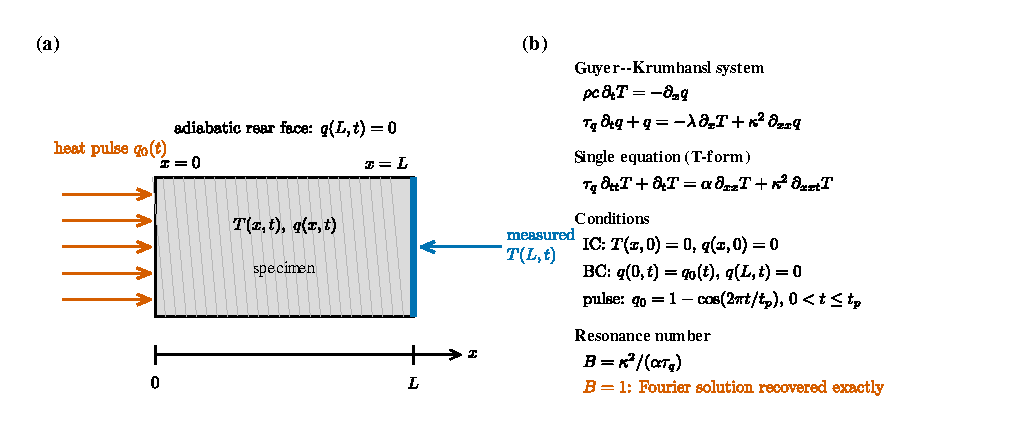
\includegraphics[width=\textwidth]{fig01_geometry.pdf}
  \caption{Problem definition. (a) The specimen is a one-dimensional slab of thickness $L$. The heat pulse $q_0(t)$ is applied at $x=0$, the rear face $x=L$ is adiabatic, $q(L,t)=0$, and the observable is the rear-face history $T(L,t)$. The geometry is genuinely one-dimensional; no lateral or curvilinear dimension enters the model. (b) The Guyer--Krumhansl system, its single-equation $T$-form, the initial and boundary conditions, the pulse shape, and the resonance number $\Bnum=\kk/(\alpha\tq)$ at which the Fourier solution is recovered exactly.}
  \label{fig:geometry}
\end{figure}


The excitation and boundary conditions are those of the validated anchor
problem \cite{Kovacs2018} and are reproduced without modification. The
irradiated face $x=0$ receives a pulse of finite duration $t_{p}$,
%
\begin{equation}
  q(0,t) =
  \begin{cases}
    q_{\max}\left[\,1 - \cos\!\left(\dfrac{2\pi t}{t_{p}}\right)\right],
      & 0 < t \leq t_{p}, \\[2ex]
    0, & t > t_{p},
  \end{cases}
  \label{eq:pulse}
\end{equation}
%
where $q_{\max}$ is the amplitude. The rear face is adiabatic for all time,
%
\begin{equation}
  q(L,t) = 0 ,
  \label{eq:bc-rear}
\end{equation}
%
and the slab starts in equilibrium with its surroundings,
%
\begin{equation}
  T(x,0) = T_{0}, \qquad q(x,0) = 0,
  \qquad \frac{\partial q}{\partial t}(x,0) = 0 ,
  \label{eq:ic}
\end{equation}
%
the last of these following from \eqref{eq:ic-derived} as required by
\cref{rem:ic} rather than being imposed. Cooling at the boundaries is
neglected, as in the anchor \cite{Kovacs2018}. The observable is the rear face
temperature history $T(L,t)$, which is the quantity recorded in a flash
experiment and the only data used in the inverse problem of
\cref{sec:practical}.


\subsection{Nondimensionalisation}
\label{sec:model-nondim}

The scaling is that of the anchor \cite{Kovacs2018}, reproduced here in full so
that every coefficient can be checked. Introduce
%
\begin{equation}
  \hat{t} = \frac{\alpha t}{L^{2}}, \qquad
  \hat{x} = \frac{x}{L}, \qquad
  \hat{T} = \frac{T - T_{0}}{T_{\mathrm{end}} - T_{0}}, \qquad
  \hat{q} = \frac{q}{\bar{q}_{0}} ,
  \label{eq:scaling}
\end{equation}
%
in which the time averaged pulse flux and the adiabatic end temperature are
%
\begin{equation}
  \bar{q}_{0} = \frac{1}{t_{p}}\int_{0}^{t_{p}} q(0,t)\,\mathrm{d}t
             = q_{\max},
  \qquad
  T_{\mathrm{end}} = T_{0} + \frac{\bar{q}_{0} t_{p}}{\rho c L} .
  \label{eq:Tend}
\end{equation}
%
The value $\bar{q}_{0} = q_{\max}$ follows because the cosine in
\eqref{eq:pulse} integrates to zero over a full period. $T_{\mathrm{end}}$ is
the temperature the insulated slab reaches once the deposited energy
$\bar{q}_{0} t_{p}$ per unit area has spread uniformly, so $\hat{T} \to 1$ as
$\hat{t}\to\infty$. The material parameters scale as
%
\begin{equation}
  \hat{\tau}_{\Delta} = \frac{\alpha t_{p}}{L^{2}}, \qquad
  \hat{\tau}_{q} = \frac{\alpha \tq}{L^{2}}, \qquad
  \hat{\kappa}^{2} = \frac{\kk}{L^{2}} ,
  \label{eq:param-scaling}
\end{equation}
%
where $\hat{\tau}_{\Delta}$ is the dimensionless pulse length. Substituting
\eqref{eq:scaling} and \eqref{eq:param-scaling} into \eqref{eq:energy} and
\eqref{eq:gk} and dropping the hats gives the dimensionless system
%
\begin{align}
  \tau_{\Delta}\, \frac{\partial T}{\partial t}
    + \frac{\partial q}{\partial x} &= 0 ,
  \label{eq:nd-energy} \\[1ex]
  \tq \, \frac{\partial q}{\partial t} + q
    + \tau_{\Delta} \, \frac{\partial T}{\partial x}
    - \kk \, \frac{\partial^{2} q}{\partial x^{2}} &= 0 ,
  \label{eq:nd-gk}
\end{align}
%
on $0 \leq x \leq 1$, with
%
\begin{equation}
  q(0,t) =
  \begin{cases}
    1 - \cos\!\left(\dfrac{2\pi t}{\tau_{\Delta}}\right),
      & 0 < t \leq \tau_{\Delta}, \\[2ex]
    0, & t > \tau_{\Delta},
  \end{cases}
  \qquad q(1,t) = 0 ,
  \label{eq:nd-bc}
\end{equation}
%
and $T(x,0) = q(x,0) = \partial_{t} q(x,0) = 0$. Eliminating $T$ as in
\cref{sec:model-reduction} gives the dimensionless counterpart of
\eqref{eq:gk-flux},
%
\begin{equation}
  \tq \, \frac{\partial^{2} q}{\partial t^{2}}
  + \frac{\partial q}{\partial t}
  = \frac{\partial^{2} q}{\partial x^{2}}
  + \kk \, \frac{\partial^{3} q}{\partial t \, \partial x^{2}} .
  \label{eq:nd-flux}
\end{equation}

Two consequences of \eqref{eq:param-scaling} are used later and are recorded
here. First, the scaling sets the dimensionless diffusivity identically to
unity, so $\alpha$ is absorbed into the time variable and cannot be read off
from the shape of a dimensionless curve; it is recovered only through the
physical time axis. Second, the dimensionless parameters
$\hat{\tau}_{q}$ and $\hat{\kappa}^{2}$ both depend on $L$, so a single
specimen thickness fixes them jointly. \Cref{tab:parameters} collects the
symbols, their dimensions and their scaled counterparts.
\begin{table}[htbp]
  \centering
  \caption{Model parameters, dimensions and scaled counterparts. The
           dimensionless diffusivity is unity by construction of
           \eqref{eq:scaling}.}
  \label{tab:parameters}
  \small
  \begin{tabular}{@{}llll@{}}
    \toprule
    \textbf{Symbol} & \textbf{Meaning} & \textbf{Dimension} &
    \textbf{Dimensionless form} \\
    \midrule
    $T$        & temperature            & \si{\kelvin}
               & $(T-T_{0})/(T_{\mathrm{end}}-T_{0})$ \\
    $q$        & heat flux              & \si{\watt\per\metre\squared}
               & $q/\bar{q}_{0}$ \\
    $x$        & position               & \si{\metre}   & $x/L$ \\
    $t$        & time                   & \si{\second}  & $\alpha t/L^{2}$ \\
    $L$        & slab thickness         & \si{\metre}   & $1$ \\
    $\rho c$   & volumetric heat capacity
               & \si{\joule\per\metre\cubed\per\kelvin} & not applicable \\
    $\lambda$  & thermal conductivity
               & \si{\watt\per\metre\per\kelvin}        & not applicable \\
    $\alpha$   & thermal diffusivity
               & \si{\metre\squared\per\second}         & $1$ \\
    $\tq$      & flux relaxation time   & \si{\second}
               & $\alpha \tq/L^{2}$ \\
    $\kk$      & nonlocal coefficient   & \si{\metre\squared}
               & $\kk/L^{2}$ \\
    $t_{p}$    & pulse duration         & \si{\second}
               & $\tau_{\Delta} = \alpha t_{p}/L^{2}$ \\
    $\Bnum$    & Fourier-resonance number & $1$ & $\Bnum$ (invariant) \\
    $s$        & Laplace variable       & \si{\per\second} & conjugate to $\hat{t}$ \\
    $m(s)$     & propagation factor     & \si{\per\metre}  & conjugate to $\hat{x}$ \\
    \bottomrule
  \end{tabular}
\end{table}


\subsection{The Fourier-resonance number}
\label{sec:model-B}

The ratio that organises the whole analysis is
%
\begin{equation}
  \Bnum = \frac{\kk}{\alpha \tq} .
  \label{eq:Bdef}
\end{equation}
%
It is dimensionless: $[\kk] = \si{\metre\squared}$,
$[\alpha] = \si{\metre\squared\per\second}$ and $[\tq] = \si{\second}$, so the
quotient has dimension $\si{\metre\squared}/(\si{\metre\squared\per\second}
\cdot \si{\second}) = 1$. Written in the scaled variables of
\eqref{eq:param-scaling}, and recalling that the dimensionless diffusivity is
unity,
%
\begin{equation}
  \frac{\hat{\kappa}^{2}}{1 \cdot \hat{\tau}_{q}}
  = \frac{\kk/L^{2}}{\alpha \tq/L^{2}}
  = \frac{\kk}{\alpha \tq}
  = \Bnum ,
  \label{eq:B-invariance}
\end{equation}
%
so $\Bnum$ takes the same value in dimensional and dimensionless variables.
The slab thickness cancels identically. This scale invariance is used in
\cref{sec:design}: within the present one dimensional model, changing the
specimen thickness does not move $\Bnum$, and multiple thicknesses of one
material share a single value of it.

The quantity $\Bnum$ measures the size of the nonlocal contribution relative to
the relaxation contribution. It is not introduced here for the first time: the
ratio $\kk/(\alpha\tq)$ is the quantity Feh\'er and Kov\'acs restrict to the
interval $1 \leq \Bnum < 3$ when fitting heat pulse data
\cite{FeherKovacs2021}, and the condition $\kk/\tq = \alpha$ appears in the
anchor \cite{Kovacs2018}. The symbol $\Bnum$ is adopted here for compactness.

\subsection{Laplace-domain formulation}
\label{sec:model-laplace}

Let $\hat{f}(x,s) = \int_{0}^{\infty} f(x,t)\,\mathrm{e}^{-st}\,\mathrm{d}t$
denote the Laplace transform. Applying it to \eqref{eq:nd-energy} and
\eqref{eq:nd-gk} with the homogeneous initial conditions \eqref{eq:ic} gives
%
\begin{align}
  \tau_{\Delta}\, s\, \hat{T} + \hat{q}^{\,\prime} &= 0 ,
  \label{eq:lap-energy} \\[0.5ex]
  \tq s\, \hat{q} + \hat{q}
    + \tau_{\Delta}\, \hat{T}^{\,\prime}
    - \kk \, \hat{q}^{\,\prime\prime} &= 0 ,
  \label{eq:lap-gk}
\end{align}
%
where a prime denotes $\partial/\partial x$. Differentiating
\eqref{eq:lap-energy} gives
$\tau_{\Delta} s \hat{T}^{\,\prime} = -\hat{q}^{\,\prime\prime}$, that is
$\tau_{\Delta}\hat{T}^{\,\prime} = -\hat{q}^{\,\prime\prime}/s$. Substituting
into \eqref{eq:lap-gk},
%
\begin{equation}
  (1 + \tq s)\,\hat{q}
  - \frac{\hat{q}^{\,\prime\prime}}{s}
  - \kk\, \hat{q}^{\,\prime\prime} = 0
  \qquad\Longleftrightarrow\qquad
  \hat{q}^{\,\prime\prime} = m^{2}(s)\, \hat{q} ,
  \label{eq:helmholtz}
\end{equation}
%
with the propagation factor
%
\begin{equation}
  m^{2}(s) = \frac{s\,(1 + \tq s)}{\alpha + \kk s} .
  \label{eq:m2}
\end{equation}
%
\Cref{eq:m2} is written with $\alpha$ retained explicitly, so that it holds in
both the dimensional and the dimensionless reading; in the scaling of
\eqref{eq:param-scaling} one sets $\alpha = 1$. The square root
$m(s) = \sqrt{m^{2}(s)}$ is taken with the principal branch,
$\operatorname{Re} m > 0$, which is the branch that keeps the solution bounded
as the slab thickness grows and is the one required for the inversion contour
used in \cref{sec:methods}. Since $\tq, \kk, \alpha > 0$, the zeros and poles
of $m^{2}$ lie on the negative real axis at $s = -1/\tq$ and $s = -\alpha/\kk$
respectively, so the principal branch is analytic in the right half plane.

Solving \eqref{eq:helmholtz} with the transformed boundary conditions
$\hat{q}(0,s) = \hat{Q}_{0}(s)$ and $\hat{q}(1,s) = 0$ gives
$\hat{q}(x,s) = \hat{Q}_{0}(s)\,\sinh\!\left[m(1-x)\right]/\sinh m$, and
recovering the temperature from \eqref{eq:lap-energy} through
$\hat{T} = -\hat{q}^{\,\prime}/(\tau_{\Delta} s)$ yields
%
\begin{equation}
  \hat{T}(x,s)
  = \frac{m\,\hat{Q}_{0}(s)\,\cosh\!\left[m\,(1-x)\right]}
         {\tau_{\Delta}\, s\, \sinh m } ,
  \label{eq:That}
\end{equation}
%
and, at the observed rear face $x=1$,
%
\begin{equation}
  \hat{T}(1,s)
  = \frac{m\,\hat{Q}_{0}(s)}
         {\tau_{\Delta}\, s\, \sinh m } .
  \label{eq:That-rear}
\end{equation}
%
The transform of the pulse \eqref{eq:nd-bc} is
%
\begin{equation}
  \hat{Q}_{0}(s)
  = \frac{\omega^{2}\left(1 - \mathrm{e}^{-s\tau_{\Delta}}\right)}
         {s\left(s^{2} + \omega^{2}\right)} ,
  \qquad \omega = \frac{2\pi}{\tau_{\Delta}} .
  \label{eq:Q0}
\end{equation}
%
The factor $1 - \mathrm{e}^{-s\tau_{\Delta}}$ vanishes at $s = \pm\mathrm{i}
\omega$, so the apparent poles of \eqref{eq:Q0} there are removable and
$\hat{Q}_{0}$ is analytic on the imaginary axis. This is not merely a formal
observation: \cref{sec:methods} shows that a numerical inversion which
separates the two factors reintroduces those poles and fails at a predictable
time.

\Cref{eq:m2,eq:That,eq:That-rear} are the objects the rest of the paper
analyses. The parameters $\tq$ and $\kk$ enter the observable
\eqref{eq:That-rear} only through $m(s)$, and $\hat{Q}_{0}$ depends on neither.
This structure is what makes the resonance analysis of \cref{sec:structural}
exact and independent of the pulse shape.

\subsection{Fourier, MCV and Nyíri limits}
\label{sec:model-limits}

Each competing model used in \cref{sec:modelselection} is an exact special case
of \eqref{eq:m2}, obtained by constraining the parameters rather than by
changing the solver. Taking limits directly in \eqref{eq:m2}:
%
\begin{align}
  \text{Fourier } (\tq \to 0,\ \kk \to 0): &\qquad
    m^{2}(s) \to \frac{s}{\alpha} ,
  \label{eq:lim-fourier} \\[0.5ex]
  \text{MCV } (\kk \to 0,\ \tq > 0): &\qquad
    m^{2}(s) \to \frac{s\,(1 + \tq s)}{\alpha} ,
  \label{eq:lim-mcv} \\[0.5ex]
  \text{Nyíri } (\tq \to 0,\ \kk > 0): &\qquad
    m^{2}(s) \to \frac{s}{\alpha + \kk s} .
  \label{eq:lim-nyiri}
\end{align}
%
\Cref{eq:lim-fourier} is the transform of the diffusion equation, for which the
response is governed by $\alpha$ alone. \Cref{eq:lim-mcv} is the
Maxwell--Cattaneo--Vernotte limit: the extra factor $(1+\tq s)$ is quadratic in
$s$, corresponding to the hyperbolic equation $\tq \partial_{tt}T +
\partial_{t}T = \alpha \partial_{xx}T$ and to a finite propagation speed
$\sqrt{\alpha/\tq}$, so this limit produces a travelling front rather than a
diffusive rise. \Cref{eq:lim-nyiri} retains the nonlocal term alone
\cite{Nyiri1991}; it is included in the model comparison because it isolates
the mechanism that MCV omits, and it is retained for that reason only. Each
limit is dimensionally consistent, since $[m^{2}] = \si{\per\metre\squared}$ in
every case. The Maxwell--Cattaneo--Vernotte and Nyíri forms therefore test the
two mechanisms of the Guyer--Krumhansl model separately, which is what makes
the comparison in \cref{sec:modelselection} a like for like one. Models
requiring a variable absent from \eqref{eq:m2} are excluded from that
comparison, as explained there.

\subsection{The resonance condition}
\label{sec:model-resonance}

Setting $\Bnum = 1$ in \eqref{eq:Bdef} gives
%
\begin{equation}
  \Bnum = 1
  \quad\Longleftrightarrow\quad
  \kk = \alpha \tq ,
  \label{eq:resonance-condition}
\end{equation}
%
which is the Fourier resonance condition. It is established in the
Guyer--Krumhansl literature: it is described as a hierarchical resonance at
which the solutions of the coupled system may coincide with those of the single
Fourier equation \cite{FulopKovacsVan2015}, it is named as the Fourier
resonance and stated in the form $\kk/\tq = \alpha$ in the anchor
\cite{Kovacs2018}, and the same coincidence is described as the Fourier
solutions being covered by the Guyer--Krumhansl solutions
\cite{Fulop2018entropy}. It is not claimed as a result of the present work.
Its consequences for the recoverability of $\tq$ and $\kk$ from a measured
temperature history are derived in \cref{sec:structural}, and no part of that
derivation is anticipated here.

\subsection{Parameterisation}
\label{sec:model-param}

The forward model is defined by the parameter vector
%
\begin{equation}
  \bm{\theta} = (\alpha,\ \tq,\ \kk) ,
  \label{eq:theta}
\end{equation}
%
which is the set an evaluation procedure is normally asked to return. For the
analysis it is convenient to use the equivalent set
%
\begin{equation}
  (\alpha,\ \tq,\ \kk)
  \ \longmapsto\
  (\alpha,\ \tq,\ \Bnum) ,
  \qquad
  \kk = \alpha\, \tq\, \Bnum ,
  \label{eq:reparam}
\end{equation}
%
the inverse transformation being immediate from \eqref{eq:Bdef}. The map is a
smooth bijection on the positive octant $\alpha, \tq, \kk > 0$, with Jacobian
determinant $\partial \kk/\partial \Bnum = \alpha \tq \neq 0$, so no
information is created or destroyed by the change of variables. Its usefulness
is that the resonance \eqref{eq:resonance-condition} becomes the single
coordinate hyperplane $\Bnum = 1$ rather than a curved surface in
$(\tq, \kk)$ space, which makes the degeneracy analysed in
\cref{sec:structural} explicit in the coordinates themselves. A change of
variables of this kind is a standard device and is not presented as a
contribution; what \cref{sec:practical} reports is the quantitative behaviour
of the estimation problem in these coordinates.

\subsection{Correspondence with the validation anchor}
\label{sec:model-anchor}

Because \cref{sec:validation} reproduces published figures, the correspondence
between the present notation and that of the anchor must be exact.
\Cref{tab:notation} states it. The dimensionless system
\eqref{eq:nd-energy}--\eqref{eq:nd-flux} is the anchor's system, the scaling
\eqref{eq:scaling}--\eqref{eq:param-scaling} is the anchor's scaling, and the
boundary and initial conditions \eqref{eq:nd-bc} are the anchor's conditions.
The anchor solves the problem by eigenfunction expansion; the present work
solves the same problem in the Laplace domain and by finite differences, as
described in \cref{sec:methods}, which is why \eqref{eq:m2} does not appear in
the anchor even though the problem it describes is the same. The governing
equation \eqref{eq:gk-flux} is linear and constant-coefficient, so an
eigenfunction solution exists for any fixed parameter set and is exactly what
the anchor computes; the choice made here is not dictated by any difficulty of
the forward problem itself. It is dictated by the inverse problem: the
identifiability analysis of \cref{sec:structural,sec:practical} and the model
comparison of \cref{sec:modelselection} require the solution and its analytic
derivatives with respect to $(\alpha,\tq,\kk)$ at a large number of parameter
combinations, whereas an eigenfunction series has eigenvalues defined only
implicitly, by a transcendental characteristic equation in those same
parameters, and differentiating the series term by term with respect to them
is correspondingly indirect. The Laplace-domain transfer function
\eqref{eq:m2} is a closed-form rational function of $(\alpha,\tq,\kk)$ and
differentiates in closed form at the same cost as the solution itself
(\cref{sec:methods-sens}), which is what the repeated evaluation underlying
\cref{sec:practical,sec:modelselection} requires. Equation numbers
are not cross referenced between the two documents, because the version of
record and the open preprint of the anchor number their equations differently;
statements are attributed to the source as a whole.



%======================================================================
\section{Analytical Structural Identifiability}
\label{sec:structural}

The consequence of the resonance condition
\eqref{eq:resonance-condition} for the inverse problem is derived below. The result is exact and
is obtained analytically from the formulation of \cref{sec:model}; the
numerical work reported later confirms it but plays no part in establishing it.

\subsection{Definition of structural identifiability}
\label{sec:struct-defs}

\begin{definition}[Structural identifiability]
\label{def:struct}
Let $\mathcal{M}(\bm{\theta})$ denote the map from a parameter vector
$\bm{\theta}$ to the noise free observable, here the rear face temperature
history. A component or combination of $\bm{\theta}$ is structurally
identifiable if $\mathcal{M}(\bm{\theta}_{1}) = \mathcal{M}(\bm{\theta}_{2})$
for all times implies that the component agrees in $\bm{\theta}_{1}$ and
$\bm{\theta}_{2}$. Structural non-identifiability is a property of the model
and the observation operator alone: it cannot be removed by reducing noise or
by sampling more densely.
\end{definition}

Practical identifiability, which concerns estimation to a stated precision from
finite noisy data, is a separate matter and is treated in
\cref{sec:practical}. The two are kept distinct throughout.

\subsection{Cancellation on the resonance ray}
\label{sec:struct-cancel}

\begin{proposition}[Fourier-equivalence of the propagation factor]
\label{prop:cancel}
For $\alpha, \tq > 0$, the condition $\Bnum = 1$ is equivalent to
$\kk = \alpha\tq$, and under it the propagation factor \eqref{eq:m2} reduces
identically to that of the Fourier equation:
%
\begin{equation}
  m^{2}(s)\big|_{\Bnum=1}
  = \frac{s\,(1+\tq s)}{\alpha + \alpha \tq s}
  = \frac{s\,(1+\tq s)}{\alpha\,(1 + \tq s)}
  = \frac{s}{\alpha} ,
  \qquad \text{for all } s .
  \label{eq:cancel}
\end{equation}
\end{proposition}

\begin{proof}
Substituting $\kk = \alpha\tq$ into the denominator of \eqref{eq:m2} gives
$\alpha + \kk s = \alpha(1 + \tq s)$. Since $\tq > 0$, the factor
$(1 + \tq s)$ is not identically zero and cancels against the identical factor
in the numerator, leaving $s/\alpha$. The cancellation is algebraic and holds
for every $s$ in the domain of analyticity, not asymptotically or
approximately.
\end{proof}

The single factor $(1+\tq s)$ carries the entire dependence of $m^{2}$ on the
relaxation time. When it cancels, $\tq$ disappears from the propagation factor,
and with it from every quantity built on the propagation factor. Comparison
with \eqref{eq:lim-fourier} shows that \eqref{eq:cancel} is exactly the Fourier
propagation factor, which is the analytical content of the known resonance
\cite{FulopKovacsVan2015,Kovacs2018,Fulop2018entropy}.

\subsection{Independence of the observable from the relaxation time}
\label{sec:struct-indep}

\begin{proposition}[Structural non-identifiability of $(\tq,\kk)$]
\label{prop:main}
Consider the Guyer--Krumhansl system of \cref{sec:model} with
$\kk = \alpha\tq$, $\alpha$ fixed. Then:
\begin{enumerate}
  \item the temperature response $T(x,t)$ is independent of $\tq$ at every
        position $x \in [0,1]$ and every time $t$, for any pulse
        $\hat{Q}_{0}(s)$;
  \item consequently the one parameter family
        $\{(\alpha, \tq, \alpha\tq) : \tq > 0\}$ produces identical
        observations, so $\tq$ and $\kk$ are not separately structurally
        identifiable in the sense of \cref{def:struct};
  \item the parameter sensitivities are exactly anti-parallel,
        %
        \begin{equation}
          \frac{\partial T}{\partial \tq}
          = -\,\alpha\, \frac{\partial T}{\partial \kk} ,
          \label{eq:antiparallel}
        \end{equation}
        %
        so the sensitivity matrix with respect to $(\tq,\kk)$ has rank one,
        the associated Fisher information matrix is singular, and the
        correlation between the two parameters is $-1$.
\end{enumerate}
\end{proposition}

\begin{proof}
\emph{(i)} By \eqref{eq:That}, the parameters $\tq$ and $\kk$ enter
$\hat{T}(x,s)$ only through $m(s)$, since $\hat{Q}_{0}$ depends on the pulse
alone and $\tau_{\Delta}$ and $s$ are independent of them. By
\cref{prop:cancel}, $m^{2}|_{\Bnum=1} = s/\alpha$, hence
$m|_{\Bnum=1} = \sqrt{s/\alpha}$ on the principal branch, which contains no
$\tq$. Therefore
%
\begin{equation}
  \hat{T}(x,s)\big|_{\Bnum=1}
  = \frac{\hat{Q}_{0}(s)\,\sqrt{s/\alpha}\,
          \cosh\!\left[\sqrt{s/\alpha}\,(1-x)\right]}
         {\tau_{\Delta}\, s\, \sinh\!\sqrt{s/\alpha}} ,
  \label{eq:That-resonance}
\end{equation}
%
which is manifestly free of $\tq$, so
$\partial \hat{T}/\partial \tq |_{\Bnum=1} \equiv 0$ for all $s$ and all
$x\in[0,1]$. The Laplace transform is injective on continuous functions, so
the same holds for $T(x,t)$ at every $t$.

\emph{(ii)} Immediate from (i): varying $\tq$ while holding
$\kk = \alpha\tq$ traces the stated one parameter family, along which the
observable is constant. The map $\mathcal{M}$ is therefore not injective.

\emph{(iii)} Write $\hat{T} = G(m)$ with
$G(m) = \hat{Q}_{0} m \cosh[m(1-x)]/(\tau_{\Delta} s \sinh m)$. By the chain
rule $\partial \hat{T}/\partial p = G'(m)\,\partial m/\partial p$ for
$p \in \{\tq, \kk\}$, so wherever $G'(m) \neq 0$ the ratio of sensitivities
depends only on $m$:
%
\begin{equation}
  \frac{\partial \hat{T}/\partial \tq}
       {\partial \hat{T}/\partial \kk}
  = \frac{\partial m/\partial \tq}{\partial m/\partial \kk} .
  \label{eq:ratio-chain}
\end{equation}
%
Differentiating \eqref{eq:m2},
%
\begin{equation}
  \frac{\partial m}{\partial \tq} = \frac{s^{2}}{2m\,(\alpha + \kk s)} ,
  \qquad
  \frac{\partial m}{\partial \kk} = -\,\frac{m\,s}{2\,(\alpha + \kk s)} ,
  \label{eq:dm}
\end{equation}
%
whence the ratio \eqref{eq:ratio-chain} equals $-s/m^{2}$ in general.
Substituting $m^{2} = s/\alpha$ from \cref{prop:cancel} gives the value
$-\alpha$, independent of $s$ and of $x$. Because the ratio is the same
constant at every $s$, it is the same constant at every $t$ after inversion,
which is \eqref{eq:antiparallel}. Stacking the sensitivities evaluated at the
observation times into a matrix
$J = [\,\partial T/\partial \tq \;\; \partial T/\partial \kk\,]$, the two
columns satisfy $J_{:,1} = -\alpha J_{:,2}$, so $\operatorname{rank} J = 1$ and
$J\,(1,\ \alpha)^{\!\top} = \bm{0}$. The Fisher information matrix for
independent Gaussian errors of variance $\sigma^{2}$ is
$F = J^{\!\top} J/\sigma^{2}$, which inherits the rank deficiency, so
$\det F = 0$ and the implied correlation is $-1$.
\end{proof}

Three features of \cref{prop:main} deserve emphasis. First, it holds for any
pulse: $\hat{Q}_{0}(s)$ cancels from the ratio \eqref{eq:ratio-chain}, so no
choice of excitation waveform restores identifiability. Second, it holds at
every interior position, not only at the rear face, so moving or adding
thermometers within the slab does not help. Third, the null direction
$(1,\alpha)$ in the $(\tq,\kk)$ plane is precisely the tangent to the ray
$\kk = \alpha\tq$, confirming that the flat direction of the likelihood is the
resonance ray itself.

\subsection{Identifiable parameter combinations}
\label{sec:struct-remains}

\cref{prop:main} is a statement about the pair $(\tq, \kk)$ and must not be
read more broadly. The diffusivity $\alpha$ is unaffected: by
\eqref{eq:That-resonance} the response at resonance is exactly a Fourier
response with diffusivity $\alpha$, and a Fourier response determines $\alpha$
from the physical time axis. Likewise the combination $\Bnum$ remains
meaningful, since the statement $\Bnum = 1$ is itself an identified fact about
the data. In the parameterisation \eqref{eq:reparam} the degeneracy is confined
to a single coordinate:
%
\begin{equation}
  \frac{\partial T}{\partial \tq}\bigg|_{\alpha,\,\Bnum}
  \;=\;
  \frac{\partial T}{\partial \tq}
  + \alpha \Bnum \frac{\partial T}{\partial \kk}
  \;\overset{\Bnum=1}{=}\;
  \frac{\partial T}{\partial \tq}
  + \alpha \frac{\partial T}{\partial \kk}
  \;=\; 0 ,
  \label{eq:reparam-degeneracy}
\end{equation}
%
by \eqref{eq:antiparallel}, while the derivatives with respect to $\alpha$ and
$\Bnum$ are not annihilated. The information the data carry is therefore
carried by $(\alpha, \Bnum)$, and it is the split of that information into
$\tq$ and $\kk$ separately that fails. The correct conclusion is not that
Guyer--Krumhansl parameters cannot be identified, but that the identifiable
content of a temperature record depends on where the material sits relative to
the resonance. \Cref{sec:practical} quantifies this for finite noisy data and
shows that $\alpha$ and $\Bnum$ remain well determined even at $\Bnum = 1$.

\subsection{Independent verification}
\label{sec:struct-verify}

The proof above is analytic. It was checked independently in three ways, each
of which confirms rather than establishes it. Symbolic computer algebra
applied to \eqref{eq:m2} and \eqref{eq:That} reproduces
$m^{2}|_{\Bnum=1} = s/\alpha$, returns identically zero for
$\partial \hat{T}/\partial \tq$ on the ray at arbitrary $x$, and simplifies
the sensitivity ratio at resonance to exactly $-\alpha$; the general
off resonance ratio is returned as $-s/m^{2}$, in agreement with
\eqref{eq:ratio-chain} and \eqref{eq:dm}. Evaluation in $50$ digit arithmetic
along the ray, with $\tq$ varied over five orders of magnitude, leaves the
computed response invariant to a spread below $10^{-30}$, whereas a control at
$\Bnum = 1.05$ separates by order $10^{-2}$, so the collapse is a property of
the ray and not of the arithmetic. Finally, an independent finite difference
solver that never forms a Laplace transform reproduces the same invariance.
Details of the numerical framework are given in \cref{sec:methods} and its
certification in \cref{sec:certification}. The collapse is exhibited directly in
\cref{fig:degeneracy}: three responses whose relaxation times differ by two
orders of magnitude are indistinguishable on the resonance ray, while the same
three separate at $\Bnum = 1.05$.
\begin{figure}[htbp]
  \centering
  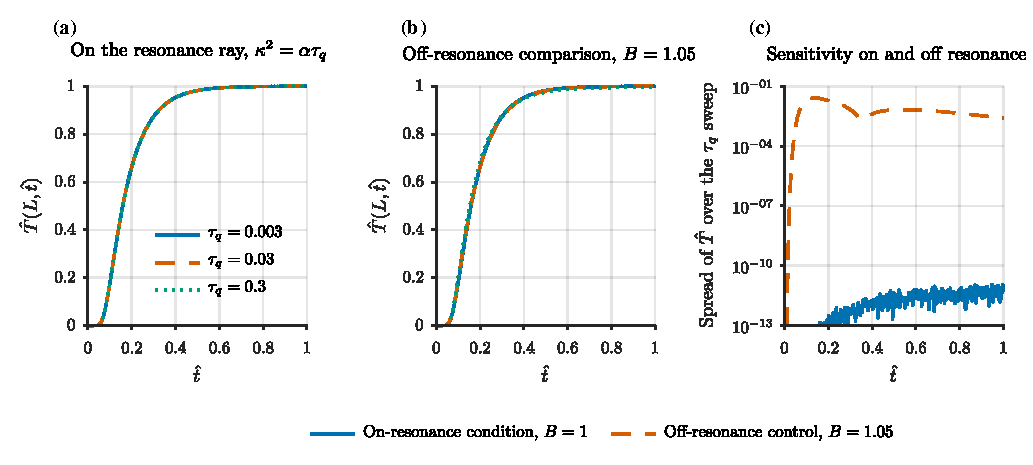
\includegraphics[width=\textwidth]{fig05_parameter_study.pdf}
  \caption{Structural degeneracy of the $(\tq,\kk)$ pair in the observable. (a) Rear-face temperature history computed along the resonance ray $\kk=\alpha\tq$, with $\tq$ varied over a factor of $100$; the three solutions are graphically indistinguishable. (b) The same sweep at the off-resonance value $\Bnum=1.05$. (c) Spread of $\hat{T}$ across the $\tq$ sweep for both conditions on a logarithmic ordinate: $1.156\times10^{-11}$ on the resonance ray against $2.595\times10^{-2}$ at the off-resonance condition, a ratio of $2.24\times10^{9}$.}
  \label{fig:degeneracy}
\end{figure}



\begin{remark}[Relation to prior work]
\label{rem:priority}
The coincidence of Guyer--Krumhansl and Fourier solutions at $\kk = \alpha\tq$
is established
\cite{FulopKovacsVan2015,Kovacs2018,Fulop2018entropy,FeherKovacs2021} and is
used here as a starting point, not offered as a finding. What
\cref{prop:main} adds is the inverse problem statement: that the coincidence
implies an exact rank deficiency of the sensitivity matrix with the explicit
null direction $(1,\alpha)$, hence a singular Fisher information matrix and the
structural non-identifiability of the pair $(\tq,\kk)$ from any temperature
observation, at any noise level and any sampling density.
\end{remark}

%======================================================================
\section{Numerical Methodology}
\label{sec:methods}

Three independent solvers of the system of \cref{sec:model} are used. Their
agreement is treated as numerical cross-checking, not as validation; external
validation is the separate exercise of \cref{sec:validation}. Every numerical
setting reported below was fixed by the convergence and stability study of
\cref{sec:certification} and is stated with its justification.

\subsection{Solver A: Laplace inversion by convolution}
\label{sec:methods-laplace}

The primary solver evaluates \eqref{eq:That-rear} numerically. A direct
inversion of \eqref{eq:That-rear} is not used, for a reason that is a result of
this work and is documented in \cref{sec:certification}. The transform
factorises as
%
\begin{equation}
  \hat{T}(1,s) = \hat{K}(s)\,\hat{Q}_{0}(s) ,
  \qquad
  \hat{K}(s) = \frac{m(s)}{\tau_{\Delta}\, s\, \sinh m(s)} ,
  \label{eq:factorisation}
\end{equation}
%
into a material kernel $\hat{K}$ and the pulse transform $\hat{Q}_{0}$ of
\eqref{eq:Q0}. As noted after \eqref{eq:Q0}, $\hat{Q}_{0}$ has removable
singularities at $s = \pm\mathrm{i}\omega$. The kernel $\hat{K}$ has none.
Accordingly the kernel alone is inverted numerically and the temperature is
recovered by the exact convolution
%
\begin{equation}
  T(1,t) = \int_{0}^{\min(t,\,\tau_{\Delta})}
           k(t-u)\, q_{0}(u)\, \mathrm{d}u ,
  \qquad
  q_{0}(u) = 1 - \cos\!\left(\frac{2\pi u}{\tau_{\Delta}}\right),
  \label{eq:convolution}
\end{equation}
%
$k$ being the inverse transform of $\hat{K}$. The integrand is analytic on the
short support $[0,\tau_{\Delta}]$, so a fixed order Gauss--Legendre rule
converges rapidly; $32$ nodes are used, at which the quadrature is converged to
better than $10^{-13}$ (doubling to $64$ nodes changes the result by at most
that amount).

The kernel is inverted by the fixed Talbot rule \cite{Talbot1979,Dingfelder2014}, which evaluates $\hat{K}$ at
the nodes
%
\begin{equation}
  s_{k} = r\,\theta_{k}\,\left(\cot\theta_{k} + \mathrm{i}\right),
  \qquad
  \theta_{k} = \frac{k\pi}{M},
  \qquad
  r = \frac{2M}{5t} .
  \label{eq:talbot-nodes}
\end{equation}
%
The number of nodes is $M = 41$. Two constraints fix this choice. The value
must be odd: at $\theta = \pi/2$, attainable only when $M$ is even, the node
lies on the imaginary axis, and \cref{sec:certification} shows that an even $M$
places a quadrature node exactly on the removable pulse pole at a predictable
time. The value must also be moderate, because the rule loses accuracy to
round off for large $M$; the accuracy plateau extends to about $M \approx 81$
and degrades beyond it. Two further implementation details are required to
avoid overflow, since $\operatorname{Re} m$ becomes large on the contour:
$1/\sinh m$ is evaluated as $2\mathrm{e}^{-m}/(1-\mathrm{e}^{-2m})$, and
$\coth m$ as $(1+\mathrm{e}^{-2m})/(1-\mathrm{e}^{-2m})$.

\subsection{Solver B: staggered-grid finite differences}
\label{sec:methods-fd}

The second solver integrates \eqref{eq:nd-energy} and \eqref{eq:nd-gk} directly
in the time domain, with no Laplace transform, so it shares no code path and no
approximation with Solver A. Temperatures are stored at $N_{x}$ cell centres
and fluxes at the $N_{x}+1$ cell faces, which places the boundary conditions
\eqref{eq:nd-bc} exactly on grid points and yields second order accurate
centred differences for both $\partial_{x} q$ and $\partial_{xx} q$. The
resulting system of ordinary differential equations is stiff, and is integrated
with a backward differentiation formula at relative tolerance $10^{-10}$ and
absolute tolerance $10^{-12}$. Production runs use $N_{x} = 400$, for which
\cref{sec:certification} reports a spatial discretisation error of order
$10^{-6}$.

\subsection{Solver C: arbitrary-precision reference}
\label{sec:methods-mp}

The third solver evaluates the same transform in arbitrary precision arithmetic
at $50$ significant digits, and serves only as a ground truth for certifying
the other two at selected probe points. Its inversion degree must be at least
$24$: at lower degree it returns a converged looking but incorrect value, an
error of about $2.5\%$ having been observed at degree $10$ near the end of the
pulse.

\subsection{Analytic sensitivities}
\label{sec:methods-sens}

All statistical quantities require the derivatives of the predicted temperature
with respect to the parameters. Finite differencing the time domain solver is
avoided, because differencing at the solver noise floor contaminates the
Jacobian and produces a spurious discrepancy between the Fisher and Monte Carlo
uncertainty estimates. The
sensitivities to $\tq$ and $\kk$, the parameters whose identifiability is at
issue, are instead obtained analytically in the Laplace domain. Differentiating
\eqref{eq:factorisation} through $m$ and using \eqref{eq:dm},
%
\begin{equation}
  \frac{\partial \hat{K}}{\partial m}
  = \frac{1}{\tau_{\Delta}\,s\,\sinh m}\left(1 - m \coth m\right),
  \qquad
  \frac{\partial \hat{K}}{\partial p}
  = \frac{\partial \hat{K}}{\partial m}\,\frac{\partial m}{\partial p},
  \qquad p \in \{\tq, \kk\} ,
  \label{eq:sens}
\end{equation}
%
and these are inverted and convolved by exactly the procedure of
\eqref{eq:convolution}. Because $\alpha$ rescales the time axis and the pulse
length rather than entering the kernel as a parameter, its sensitivity is
obtained by a central difference in $\alpha$ alone. The analytic derivatives
were verified against central differences of the forward solver, agreeing to a
maximum relative deviation of $5.3\times10^{-7}$.

\subsection{Estimation and statistical procedures}
\label{sec:methods-stats}

Parameters are estimated by Levenberg--Marquardt minimisation \cite{Najafi2024} of the sum of
squared residuals, carried out in logarithmic parameters so that positivity is
enforced automatically and the scaling of the three parameters is comparable,
with the analytic Jacobian of \cref{sec:methods-sens}. Synthetic observations
are generated by adding independent Gaussian noise of standard deviation
$\sigma = \eta\,(T_{\max}-T_{\min})$ to the noise free response, with
$\eta = 2\%$ unless stated otherwise.

Four diagnostics are used, and are reported together because each fails in a
different way near a degeneracy.
The Fisher information matrix for independent Gaussian errors is
$F = J^{\!\top}J/\sigma^{2}$, with $J$ the analytic sensitivity matrix in log
parameters. Asymptotic standard errors are the square roots of the diagonal of
$F^{-1}$, and the condition number of $F$ measures the conditioning of the
estimation problem. This is the standard construction underlying
Fisher-based experimental design \cite{Neilsen2018,Chhajer2024,Liu2026}, and the
way the matrix is approximated is known to affect the resulting design
\cite{Stromberg2016}. The Fisher analysis is local and assumes a quadratic
log likelihood, so it is checked against a Monte Carlo study, in which the
estimator is applied to repeated noise realisations and the empirical spread of
the estimates recorded. Profile likelihood \cite{Raue2009,Simpson2023}, computed by fixing $\tq$ on a
grid and re optimising the remaining parameters, gives a confidence interval
valid without the quadratic assumption, using the $\chi^{2}(1)$ threshold of
$3.841$ at the $95\%$ level; workflows automating this diagnostic are now
available \cite{Borisov2026,Simpson2026}. Model selection uses the Bayesian information criterion
\cite{Weakliem1999},
$\mathrm{BIC} = n\ln(\mathrm{SSE}/n) + k \ln n$, applied to candidate models
that are exact special cases of the same transfer function
\eqref{eq:m2} so that solver, protocol and convergence criteria are identical
across models.

Because the estimation problem is poorly conditioned near resonance, the
dependence of the result on the optimiser starting point is itself studied:
starts are drawn from log normal perturbations of the true parameters at
several widths, and the spread of the recovered values is recorded separately
from the spread induced by measurement noise.

\subsection{Solution algorithm}
\label{sec:methods-algorithm}

The forward evaluation, the sensitivity evaluation and the identifiability
diagnostics are organised into the single procedure summarised in
\cref{alg:main} (\ref{app:algorithm}). The structure is dictated by two
requirements established in \cref{sec:certification}: the material kernel
must be inverted separately from the pulse transform, because the split
form fails at even Talbot node counts, and the sensitivities must be
obtained analytically rather than by finite differences, because
differencing at the solver noise floor corrupts the Fisher matrix.

Three features of the procedure are dictated by numerical requirements rather
than by convenience, and are justified below.

\emph{Kernel-only inversion (line 4).} The pulse transform $\hat{Q}_0$ has
removable singularities on the imaginary axis. When the full product is inverted
on a Talbot contour with an even number of nodes, a quadrature node coincides
with one of these singularities and the computed temperature diverges by up to
ten orders of magnitude at a predictable instant. Inverting the pole-free kernel
alone removes the failure mode entirely, and the parity dependence is documented
in \cref{fig:talbot}. Talbot's method itself \cite{Talbot1979} and its modern
refinements \cite{Dingfelder2014} are well established; the interaction with a
pulse transform carrying removable poles is what required care here. Earlier
treatments of Laplace inversion for inverse conduction \cite{Woo1981} and
analyses of inversion stability \cite{Kryzhniy2006,Zakian1969}
informed the choice of contour.

\emph{Analytic sensitivities (line 11).} Because $m^{2}(s)$ is a rational
function of $s$ with polynomial dependence on the parameters, each sensitivity
can be inverted on the same contour at the same cost as the solution itself.
Finite-difference Jacobians formed at the solver noise floor yield a systematic
discrepancy between the Fisher and Monte Carlo uncertainty estimates; with
analytic sensitivities the two estimates agree, as reported in
\cref{fig:identoverview}(d). The influence of the Fisher-matrix approximation
on the resulting inference is documented in the estimation literature
\cite{Stromberg2016}.

\emph{Profiling rather than linearised intervals (line 16).} Near the resonance
the log-likelihood ceases to be quadratic in $\tq$, so an asymptotic standard
error is no longer a meaningful summary. Profile likelihood is the standard
remedy \cite{Raue2009,Simpson2023} and is what reveals that the admissible
interval is unbounded at $\Bnum=1$ rather than merely large.

%======================================================================
\section{External Validation of the Forward Operator}
\label{sec:validation}

External validation of the forward operator against an independently
published solution is reported here. The anchor is the analytical laser flash
solution of the Guyer--Krumhansl equation published by Kov\'acs
\cite{Kovacs2018}, which solves exactly the problem set out in
\cref{sec:model} by eigenfunction expansion, independently of the methods of
\cref{sec:methods}.

\subsection{Categories of evidence}
\label{sec:val-scope}

Two categories are kept strictly separate throughout this paper.
Agreement between independent implementations of the same equations is
numerical cross-checking, not external validation. Agreement between the
present implementation and results published by another author is external
validation.
The present section reports the second; the first is reported in
\cref{sec:certification}.

A third distinction is equally important. What is validated here is the
\emph{forward operator}: the ability of the present implementation to compute
the temperature response of the Guyer--Krumhansl system given the parameters.
This validation makes no statement about the inverse problem. The
identifiability results
of \cref{sec:structural,sec:practical} are established analytically and
verified by the separate means described there, not by this reproduction. No
experimental validation of the inverse conclusions is claimed anywhere in this
paper.

\subsection{Reproduction protocol}
\label{sec:val-method}

Published figures were extracted from the anchor at native resolution
($4000 \times 1908$ pixels) and digitised by two independent passes, one taking
the intensity weighted centroid of the plotted curve band and one taking the
midpoint of its envelope. The disagreement between the passes, combined with
the curve half width, defines a digitisation noise floor
%
\begin{equation}
  \sigma_{d} = \sqrt{\;\overline{\left(\Delta_{AB}\right)^{2}}
                     \;+\; \operatorname{median}(\text{half width})^{2} } ,
  \label{eq:sigmad}
\end{equation}
%
where $\Delta_{AB}$ is the pointwise difference between the two passes. All
comparisons are reported against $\sigma_{d}$, because a reproduction cannot
meaningfully be shown to agree with a published curve to better than the
precision with which that curve can be read.

The parameters were taken exactly as printed in the anchor and are listed in
\cref{tab:validation-params}. No parameter was fitted, tuned or adjusted at any
point. The digitisation mask was refined during the extraction, since an
initial legend mask clipped the upper curve band; correcting the mask boundary
improved the agreement between the two independent passes by a factor of about
twenty five, and the corrected extraction is used throughout.
\begin{table}[htbp]
  \centering
  \caption{Parameters used for the reproduction, taken verbatim from the
           anchor \cite{Kovacs2018}. Dimensionless throughout, with
           $\tau_{\Delta}=0.04$ in every case. No value was fitted.}
  \label{tab:validation-params}
  \small
  \begin{tabular}{@{}lllll@{}}
    \toprule
    \textbf{Anchor figure} & \textbf{Regime} & $\tq$ & $\kk$ &
    \textbf{Series terms / time span} \\
    \midrule
    Fig.~2 & convergence study    & $0.02$ & $0.02$ &
      $N = 1,3,10,40$; $t\in[0,1]$ \\
    Fig.~3 & Fourier resonance    & $0.02$ & $0.02$ &
      $N = 40$; $t\in[0,1]$ \\
    Fig.~5 & over-diffusive       & $0.02$ & $0.20$ &
      $N = 10$; $t\in[0,2]$ \\
    \bottomrule
  \end{tabular}
\end{table}


\subsection{Reproduction accuracy}
\label{sec:val-results}

The first reference case is presented in \cref{fig:validation} and the second
in \cref{fig:overdiffusive}; the metrics for all three cases are collected in
\cref{tab:validation-results}. Each reproduction uses the
published parameters directly, with no fitting. The three reference cases are
three figures of a single published study \cite{Kovacs2018} rather than three
independent publications, and are described as such throughout.

The outcome is reported in \cref{tab:validation-results}, with the overlays and
residuals in \cref{fig:validation}. For the two solution
figures the reproduction error falls below the digitisation
noise floor: the residual is dominated by the precision with which the
published curves can be read, not by any discrepancy between the published
solution and the present implementation, with the great majority of residuals
falling within $\pm 2\sigma_{d}$ in both cases.
\begin{figure}[htbp]
  \centering
  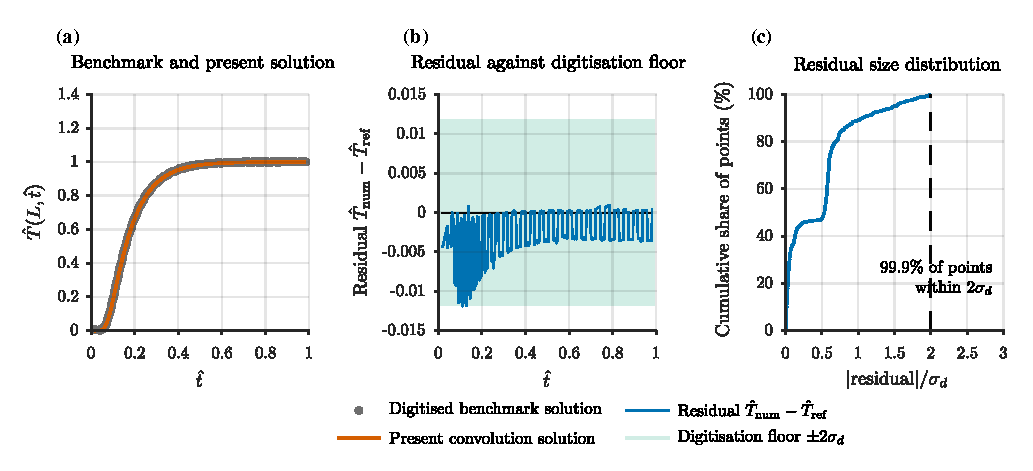
\includegraphics[width=\textwidth]{fig02_anchor_resonance.pdf}
  \caption{External validation of the forward operator against the first reference case, the resonance condition $\Bnum=1$. (a) Digitised benchmark solution read from the published figure, overlaid with the present convolution solution evaluated at the literature parameters with no fitting. (b) Residual $\hat{T}_{\mathrm{num}}-\hat{T}_{\mathrm{ref}}$ against the digitisation floor $\pm2\sigma_{d}$, where $\sigma_{d}$ is the standard deviation attributable to reading the published curve. (c) Empirical cumulative distribution of $|\text{residual}|/\sigma_{d}$, with the bound $2\sigma_{d}$ marked. Verified metrics: NRMSE $=0.384\%$, RMSE $=3.84\times10^{-3}$, $n=729$ comparison points, and $99.9\%$ of residuals within $\pm2\sigma_{d}$. External validation of the forward operator only; not validation of the inverse conclusions and not experimental validation.}
  \label{fig:validation}
\end{figure}

\begin{figure}[htbp]
  \centering
  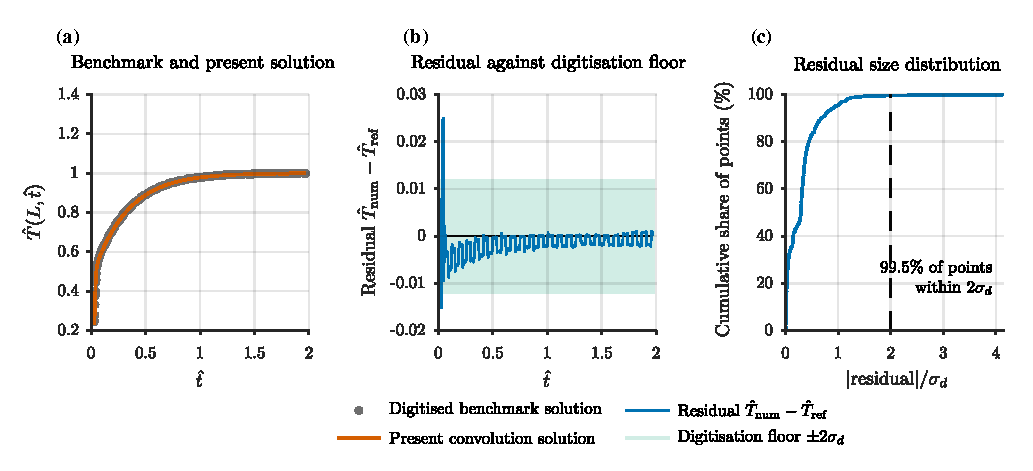
\includegraphics[width=\textwidth]{fig03_anchor_overdiffusive.pdf}
  \caption{External validation of the forward operator against the second reference case, the over-diffusive condition, using the same three-panel construction and the identical unmodified solver as \cref{fig:validation}. Panels are as in \cref{fig:validation}: (a) digitised benchmark solution and present convolution solution, (b) residual against the digitisation floor $\pm2\sigma_{d}$, (c) empirical cumulative distribution of the scaled residual. Verified metrics: NRMSE $=0.382\%$, RMSE $=2.88\times10^{-3}$, $n=743$, and $99.5\%$ of residuals within $\pm2\sigma_{d}$. The three reference cases used in this work are three figures of the single published study \cite{Kovacs2018}, not three independent publications.}
  \label{fig:overdiffusive}
\end{figure}


The convergence figure of the anchor, which shows the eigenfunction expansion
truncated at successively larger numbers of terms, is reproduced with a pooled
normalised error of $0.483\%$. One entry requires comment. The $N=40$ curve of that figure is nearly converged and spans a
temperature range of only $0.031$, so normalising its error by its own range
gives $8.19\%$ while the absolute error, $2.7\times10^{-3}$, is comparable to
the other curves. Normalised against the full range of the figure the same
residual is $0.162\%$. Both numbers are reported in
\cref{tab:validation-results}; the large value is an artefact of normalising by
a small range, not a failure of reproduction.
\begin{table}[htbp]
  \centering
  \caption{External validation of the forward operator against the published
           figures of the anchor \cite{Kovacs2018}. $\sigma_{d}$ is the
           digitisation noise floor \eqref{eq:sigmad}. A ratio
           $\mathrm{RMSE}/\sigma_{d} < 1$ means the reproduction error is
           below the precision with which the published curve can be read.
           These figures are reproductions for validation, not original
           results.}
  \label{tab:validation-results}
  \small
  \setlength{\tabcolsep}{4.2pt}
  \resizebox{\textwidth}{!}{%
  \begin{tabular}{@{}lrrrrrr@{}}
    \toprule
    \textbf{Figure} & \textbf{Points} & \textbf{RMSE} & \textbf{NRMSE} &
    $E_{\max}$ & $\sigma_{d}$ & \textbf{RMSE}$/\sigma_{d}$ \\
    \midrule
    Fig.~3 (resonance)     & 729 & 0.00384 & \SI{0.384}{\percent} &
      0.01189 & 0.00593 & 0.65 \\
    Fig.~5 (over-diffusive)& 743 & 0.00288 & \SI{0.382}{\percent} &
      0.02496 & 0.00603 & 0.48 \\
    Fig.~2 (pooled)        & 1999 & 0.00819 & \SI{0.483}{\percent} &
      0.05813 & --- & --- \\
    \quad $N=40$ subset, own range & 109 & 0.00275 &
      \SI{8.19}{\percent} & 0.01044 & --- & --- \\
    \quad $N=40$ subset, full range & 109 & 0.00275 &
      \SI{0.162}{\percent} & 0.01044 & --- & --- \\
    \bottomrule
  \end{tabular}%
  }
  \par\smallskip\footnotesize
  Entries marked --- are not applicable: the pooled convergence figure
  reports curves at several truncation levels rather than a single
  digitised trace, so a digitisation standard deviation $\sigma_{d}$ is
  not defined for it.
\end{table}




The residuals show a low amplitude sawtooth of about one pixel, consistent with
pixel quantisation of the source image, and the largest pointwise deviations
occur where the published curve rises steeply, where a small horizontal
digitisation error maps to a large vertical one. Neither feature indicates a
model discrepancy.



\subsection{Scope established by the reproduction}
\label{sec:val-interp}

The forward framework reproduces three published figures of an independently
authored analytical solution, using the published parameters without
adjustment, to within the precision with which those figures can be read. The
forward operator underlying every subsequent computation in this paper is
therefore externally validated. The inverse problem is not validated by this
exercise, and is not claimed to be.

%======================================================================
\section{Numerical Certification}
\label{sec:certification}

The numerical framework of \cref{sec:methods} resolves the quantities reported
in this paper far above its own error floor, as established below.
The agreement between solvers reported here is numerical cross-checking, not
external validation.

\subsection{Failure mode of the Laplace inversion}
\label{sec:cert-talbot}

The most consequential result of the certification concerns the numerical
Laplace inversion, for which a direct implementation of the transform admits a
parity-dependent failure mode that is not signalled by any convergence
diagnostic.

The effect is quantified in \cref{fig:talbot}. If the transform
\eqref{eq:That-rear} is
inverted by applying the fixed Talbot
rule to the material kernel and handling the pulse factor
$1-\mathrm{e}^{-s\tau_{\Delta}}$ by the second shift theorem, the computed
solution is catastrophically wrong at one isolated time, while remaining
accurate everywhere else.
\begin{figure}[htbp]
  \centering
  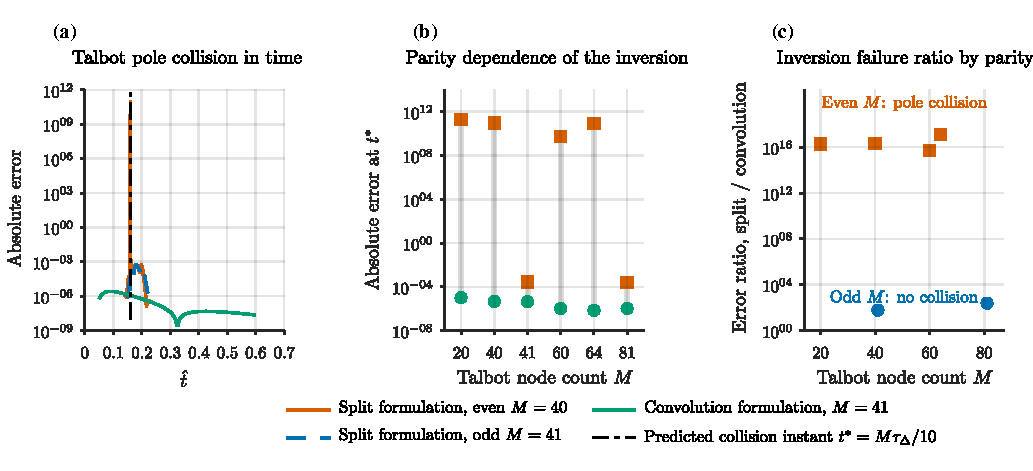
\includegraphics[width=\textwidth]{fig11_talbot_certification.pdf}
  \caption{Certification of the numerical Laplace inversion. (a) Absolute error against time for the split formulation at even node count $M=40$ and odd node count $M=41$, and for the adopted convolution formulation, with the predicted pole-collision instant $t^{*}=M\tau_{\Delta}/10$ marked. (b) Absolute error at $t=t^{*}$ for six node counts, comparing the split and convolution formulations; the connecting segments indicate the discrepancy at each $M$. (c) Ratio of the split to the convolution error, separating even from odd node counts. The split formulation fails by up to $9.7\times10^{10}$ at even $M$, whereas the convolution formulation remains at $\mathcal{O}(10^{-6})$ throughout. The failure is a property of the numerical inversion and not of the physics: the exact solution is regular at $t^{*}$. The convolution formulation with $M=41$ is used throughout this work.}
  \label{fig:talbot}
\end{figure}
 The cause is exact and predictable. The pulse
transform \eqref{eq:Q0} has removable singularities at $s=\pm\mathrm{i}\omega$,
$\omega = 2\pi/\tau_{\Delta}$, which are cancelled by the zeros of
$1-\mathrm{e}^{-s\tau_{\Delta}}$. Splitting the two factors and inverting
$\omega^{2}/[s(s^{2}+\omega^{2})]$ alone reinstates genuine poles at
$s = \pm\mathrm{i}\omega$. The Talbot contour \eqref{eq:talbot-nodes} meets the
imaginary axis only at $\theta = \pi/2$, which is a quadrature node exactly
when $M$ is even, and there $s = \mathrm{i} r \pi/2$. Setting
$r\pi/2 = \omega$ with $r = 2M/(5t)$ gives the failure time
%
\begin{equation}
  t^{\ast} = \frac{M\,\tau_{\Delta}}{10} .
  \label{eq:tstar}
\end{equation}
%
This prediction was tested directly. For $\tau_{\Delta}=0.04$ and even
$M \in \{20,40,60,64\}$ the error at $t^{\ast}$ is of order
$10^{9}$ to $10^{11}$, while at $0.98\,t^{\ast}$ and $1.02\,t^{\ast}$ it
remains of order $10^{-4}$; for odd $M=41$ no such spike occurs at any time.
The two remedies are therefore to use an odd number of nodes, which removes the
node from the imaginary axis, and better, to avoid the splitting altogether.
The convolution formulation \eqref{eq:convolution} adopted in
\cref{sec:methods-laplace} does the latter: it inverts only the pole free
kernel $\hat{K}$, so the removable singularities never appear.


Two points follow. First, this is a property of the numerical inversion, not of
the physics: the exact solution is perfectly regular at $t^{\ast}$, and nothing
physical happens there. Second, the usual remedy of increasing the number of
quadrature nodes is not merely ineffective here but actively harmful, since
$t^{\ast}$ scales with $M$ and simply moves the failure to a later time while
round off grows. With the convolution formulation the accuracy plateau extends
across $M \in [25,81]$, degrading beyond $M \approx 91$ through round off;
$M = 41$ is used throughout.

\subsection{Spatial convergence and arithmetic precision}
\label{sec:cert-conv}

\Cref{fig:convergence} collects the convergence evidence. Panels (a) and (b)
quantify the spatial discretisation error and its observed order, panel (c) the
agreement between the truncated eigenfunction series and the convolution
solution, and panel (d) the correspondence between the sampling and asymptotic
uncertainty estimates. All four are internal verification of the present
implementation; external validation is reported separately in
\cref{sec:validation}.

With the corrected formulation the certification results are as follows.
Against the arbitrary precision reference of \cref{sec:methods-mp}, the
convolution solver agrees to between $10^{-11}$ and $10^{-13}$ at times away
from the steep rise, and to about $10^{-7}$ against the independent finite
difference solver across the whole record, the latter being limited by the
finite difference discretisation rather than by the inversion. Increasing the
Gauss--Legendre order from $32$ to $64$ changes the result by at most
$10^{-13}$, so the convolution quadrature is fully converged.

The finite-difference solver converges at the expected second order in space.
Measured against a Richardson reference the observed order is $2.00$ and the
spatial error at the production resolution $N_{x}=400$ is
$2.6\times 10^{-6}$; measured against the independent $N_{x}=3200$ solution of
\cref{fig:convergence}(a) the corresponding error is $1.00\times10^{-5}$ and the
per-interval orders are $2.00$, $2.02$, $2.07$ and $2.32$. The two figures differ because they use different reference solutions, both
retained as independent checks.
\begin{figure}[htbp]
  \centering
  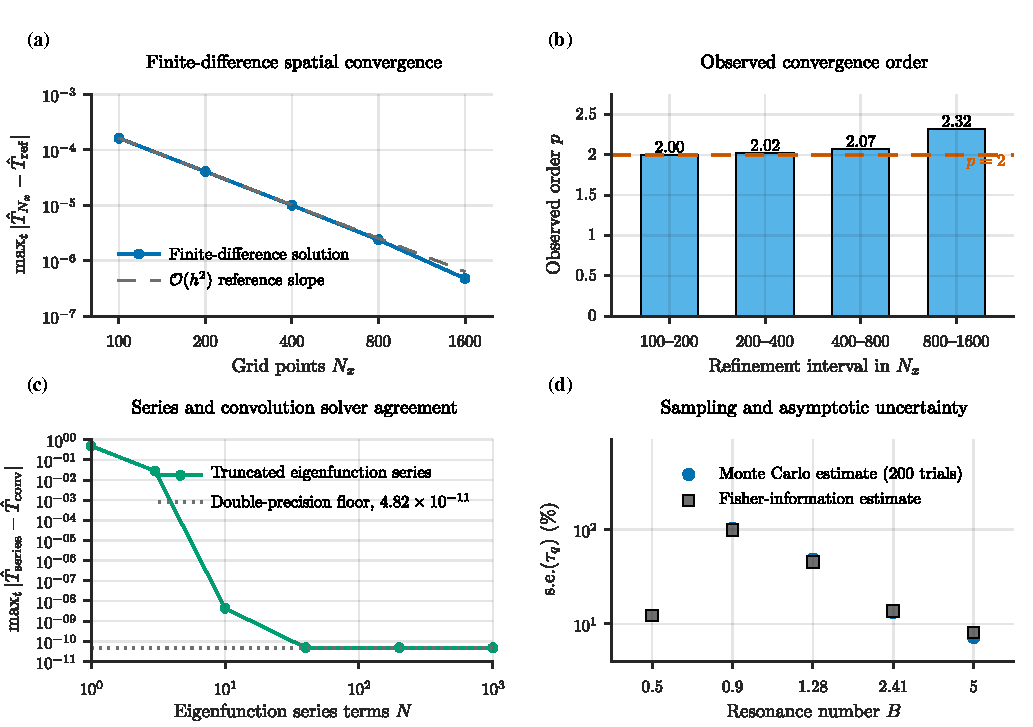
\includegraphics[width=\textwidth]{fig04_convergence_certification.pdf}
  \caption{Numerical verification of the solver and characterisation of the inverse procedure, assembled from four complementary lines of evidence. (a) Finite-difference spatial error against the grid resolution $N_x$ on logarithmic axes, measured against the $N_x=3200$ reference solution, with a second-order reference slope. (b) Observed convergence order $p$ for each successive refinement interval: $2.00$, $2.02$, $2.07$ and $2.32$, against the theoretical value $p=2$. These four values originate from the documented Windows verification run and are recorded there, and reproduced here, to four significant figures; a machine-readable subset of the same refinement ladder ($N_x=100$ to $400$), independently regenerable from the supplied pipeline, gives orders of $2.02$ and $2.07$ for its two intervals, confirming the same near-second-order behaviour without reproducing the four-value ladder digit for digit. (c) Agreement between the truncated eigenfunction series and the convolution solution against the number of retained terms $N$, descending to the double-precision floor $4.82\times10^{-11}$. (d) Monte Carlo estimate of $\mathrm{s.e.}(\tq)$ from $200$ trials against the asymptotic Fisher-information estimate at each resonance number. Panels (a)--(c) verify the numerical convergence of the present implementation and are internal cross-checking rather than external validation; panel (d) characterises the behaviour of the inverse procedure on controlled synthetic data. No panel constitutes external or experimental validation.}
  \label{fig:convergence}
\end{figure}

\begin{figure}[htbp]
  \centering
  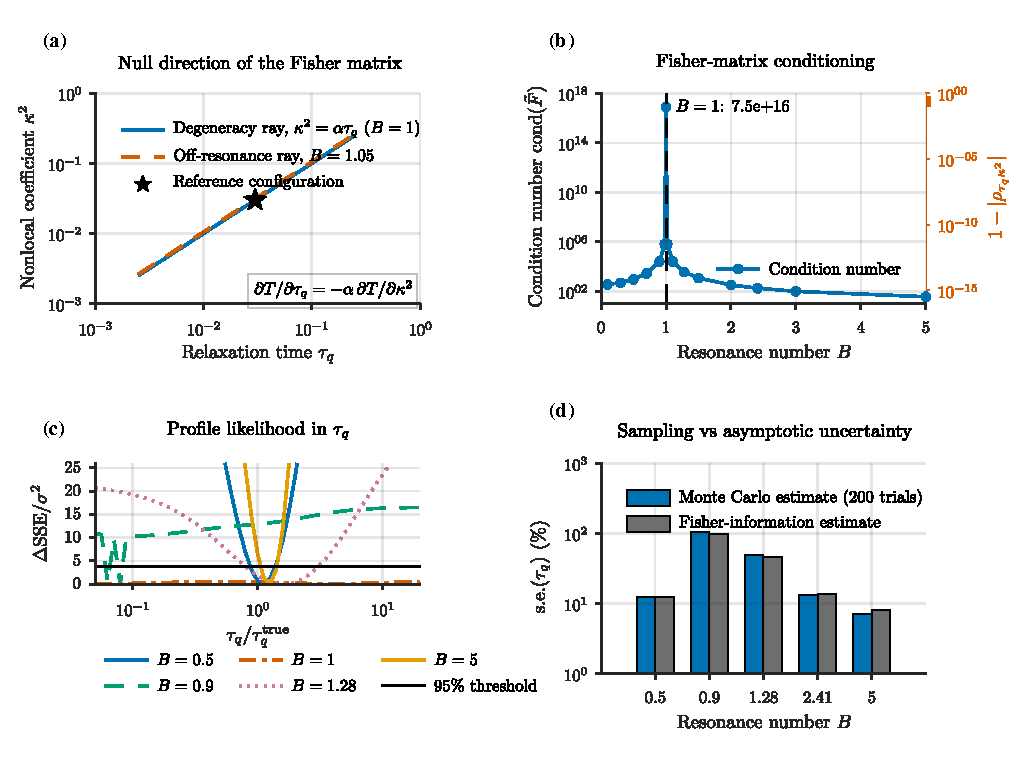
\includegraphics[width=\textwidth]{fig07_identifiability.pdf}
  \caption{Structural and practical non-identifiability of the $(\tq,\kk)$ split at the resonance condition. (a) Null direction of the Fisher matrix: the analytic degeneracy ray $\kk=\alpha\tq$ ($\Bnum=1$) along which the observable is invariant, the off-resonance ray at $\Bnum=1.05$, and the reference configuration, with the exact identity $\partial T/\partial\tq=-\alpha\,\partial T/\partial\kk$ annotated. (b) Condition number of the Fisher matrix against $\Bnum$ on a logarithmic ordinate, attaining $7.50\times10^{16}$ at $\Bnum=1$, together with the correlation deficit $1-|\rho_{\tq\kk}|$ on the right-hand axis, which collapses to $3.3\times10^{-16}$ at the same point. (c) Profile likelihood in $\tq$ at each computed resonance number, with the $95\%$ threshold from the $\chi^{2}_{1}$ distribution; the $\Bnum=0.9$ curve is multimodal because the re-optimisation at fixed $\tq$ reaches different local minima at adjacent grid nodes, and no interval is read from it. (d) Monte Carlo estimate of $\mathrm{s.e.}(\tq)$ from $200$ trials against the asymptotic Fisher-information estimate, at each computed resonance number.}
  \label{fig:identoverview}
\end{figure}

\begin{figure}[htbp]
  \centering
  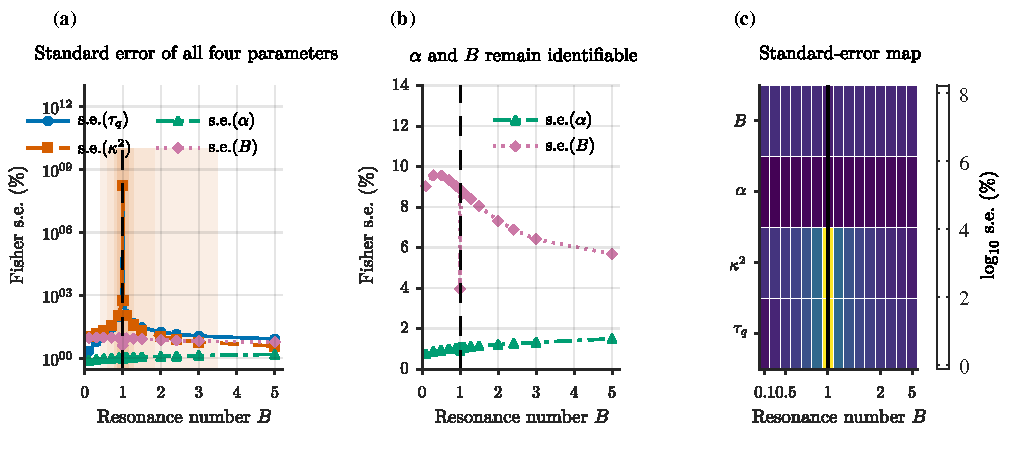
\includegraphics[width=\textwidth]{fig08_parameter_map.pdf}
  \caption{Practical identifiability as a function of the resonance number. (a) Fisher standard errors of $\tq$, $\kk$, $\alpha$ and $\Bnum$ against $\Bnum$ on a logarithmic ordinate. The shaded regions are the verified bands within which $\mathrm{s.e.}(\tq)$ exceeds $10$, $20$, $50$ and $100\%$; the $20\%$ band is $\Bnum\in[0.628,1.804]$. (b) The same standard errors for $\alpha$ and $\Bnum$ on a linear ordinate, showing that both remain small and nearly flat through resonance, $\alpha$ to approximately $1\%$ and $\Bnum$ to between $4$ and $10\%$. (c) Map of $\log_{10}\mathrm{s.e.}$ for all four parameters against $\Bnum$, with the resonance column marked. Standard errors are asymptotic and correspond to the configuration of \cref{sec:prac-config}.}
  \label{fig:identifiability}
\end{figure}
 The temporal error at relative tolerance
$10^{-10}$ is of order $10^{-9}$. Repeating the arbitrary precision
evaluation at $15$, $30$ and $50$ digits changes the result by no more than
$8.9\times10^{-16}$, confirming that double precision is sufficient and that
none of the reported quantities is limited by round off.



The eigenfunction series used by the anchor converges as $O(N^{-2})$, the ratio
of successive errors tending to $4.0$; at $N=40$ the truncation error is
$3.1\times10^{-3}$, and $N \geq 80$ is required to reach $7.8\times10^{-4}$.
This matters only for reproducing the anchor's own truncated curves in
\cref{sec:validation}, not for the present solvers.

\subsection{Limiting cases and physical admissibility}
\label{sec:cert-limits}

The limits of \cref{sec:model-limits} were checked numerically. Setting
$\kk = \alpha\tq$ reproduces the analytical Fourier solution to
$2.6\times10^{-6}$, an independent numerical confirmation of
\cref{prop:cancel}. Letting $\tq,\kk \to 0$ likewise recovers the Fourier
solution to $2.6\times10^{-6}$. The computed temperature remains non negative
throughout in every case tested, in agreement with the anchor and in contrast
to the negative temperature artefacts reported for dual phase lag models
\cite{Rukolaine2014}, and the long time limit satisfies
$T(1,t\to\infty) = 1.00000000$ as required by the normalisation
\eqref{eq:Tend}.

\subsection{Error budget}
\label{sec:cert-budget}

\Cref{tab:certification} assembles the error budget. The total numerical error
of the framework is of order $10^{-6}$, whereas the digitisation noise floor of
the external validation exercise is $6\times10^{-3}$, three orders of magnitude larger.
The external validation of \cref{sec:validation} is therefore
digitisation limited, not solver limited: the agreement reported there is as
close as the published figures permit.


%======================================================================
\section{Practical Identifiability}
\label{sec:practical}

\cref{sec:structural} established an exact degeneracy at the single point
$\Bnum = 1$. A point degeneracy would be of limited practical interest if the
estimation problem recovered quickly on either side of it. It does not: the
degeneracy extends into a wide neighbourhood within which $\tq$ cannot be
estimated to any useful precision. The quantities that remain determined in that
neighbourhood are identified below.

\subsection{Reference configuration}
\label{sec:prac-config}

All results in this section are for one stated configuration: $\tq = 0.03$,
$\tau_{\Delta} = 0.04$, $80$ observation times uniformly spaced on
$t \in [0.02, 1.2]$, independent Gaussian noise of $2\%$ of the temperature
range, estimation in log parameters with the analytic Jacobian of
\cref{sec:methods-sens}. Working units are $L=1$, $\alpha=1$, $t_{p}=0.04$.
The numerical values of the band boundaries reported below depend on this
configuration and are not universal constants. Only the singularity at
$\Bnum = 1$ is configuration independent, because it is structural.

\subsection{Fisher-information conditioning}
\label{sec:prac-landscape}

\Cref{fig:identoverview} assembles the diagnostics of the same structural
result, and \cref{fig:identifiability} maps the standard errors and
conditioning across $\Bnum$. The Fisher conditioning, the profile likelihood
and the Monte Carlo study are methodologically independent: the first uses
analytic derivatives at a point, the second re-optimises the objective along a
fixed direction, and the third samples the estimator itself. Their agreement
indicates that the degeneracy is a property of the parameter-to-observable map
rather than an artefact of any single statistical construction. The claim
remains confined to the $(\tq,\kk)$ split, since $\alpha$ and $\Bnum$ stay
identifiable throughout.

\Cref{tab:identifiability} and \cref{fig:identifiability} report the Fisher
analysis as a function of $\Bnum$. The behaviour is a smooth deterioration towards the resonance rather
than an isolated pathology. Far from resonance the problem is well conditioned:
at $\Bnum = 0.10$ the condition number of the Fisher matrix is $3.6\times10^{2}$
and the standard error on $\tq$ is $2.05\%$. As $\Bnum \to 1$ the condition
number rises by fourteen orders of magnitude, the estimator correlation between
$\tq$ and $\kk$ tends to $+1$, and the standard error on $\tq$ diverges. At
$\Bnum = 1$ the Fisher matrix is numerically singular, as \cref{prop:main}
requires.

The mechanism is the progressive alignment of the two sensitivity directions.
Away from resonance the response retains a component that distinguishes a change
in relaxation from a change in nonlocality, since the factor $(1+\tq s)$ in the
numerator of \eqref{eq:m2} and the factor $(\alpha+\kk s)$ in its denominator
act on different regions of the transform variable. As $\Bnum \to 1$ these two
factors approach proportionality and cancel in the limit, so a perturbation in
$\tq$ becomes reproducible by a compensating perturbation in $\kk$. The
observable consequence is that the rise portion of the rear-face history, which
carries most of the information about the relaxation mechanism, becomes
insensitive to the split while remaining fully sensitive to $\alpha$. This is
why the diffusivity and the resonance number stay well determined while the
individual coefficients do not.

Two correlation coefficients occur in this problem, with opposite signs. The
coefficient tabulated in
\cref{tab:identifiability}, and plotted in \cref{fig:identoverview}(b), is the
estimator correlation
\[
  \rho_{\tq\kk} = [F^{-1}]_{12}\big/\sqrt{[F^{-1}]_{11}[F^{-1}]_{22}}
\]
obtained from
the inverse Fisher matrix, which is the correlation of the sampling
distribution of the estimates and tends to $+1$ at resonance: an
overestimate of $\tq$ is compensated by an overestimate of $\kk$ along the ray
$\kk=\alpha\tq$. The coefficient $-1$ of \cref{prop:main} is the normalised
off-diagonal of the Fisher matrix itself,
$F_{12}/\sqrt{F_{11}F_{22}}$, which follows from the anti-parallel
sensitivities \eqref{eq:antiparallel}. Both express the same rank-one
degeneracy with null direction $(1,\alpha)$; the sign difference is a property
of inverting a singular two-by-two block and not a discrepancy.


The Monte Carlo results in the same table are consistent with the Fisher
predictions where the latter are valid. At $\Bnum = 0.50$ the Fisher standard error on $\tq$ is
$12.4\%$ against a Monte Carlo value of $12.4\%$; at $\Bnum = 0.90$, $98.8\%$
against $103.9\%$; at $\Bnum = 1.28$, $45.6\%$ against $48.9\%$; at
$\Bnum = 2.41$, $13.7\%$ against $13.3\%$; at $\Bnum = 5.0$, $8.1\%$ against
$7.2\%$. The two estimates agree throughout the range in which the asymptotic
approximation is meaningful, which supports the use of the Fisher standard
error as a summary statistic outside the immediate neighbourhood of the
resonance. The agreement is contingent on analytic sensitivities: Jacobians
formed by differencing the forward solver at its own noise floor produce a
spurious discrepancy between the two estimates, which is why the analytic route
of \cref{sec:methods-sens} is used throughout.

Near resonance the two diverge for a well understood reason: the log likelihood
ceases to be quadratic, so the asymptotic Fisher standard error is no longer a
meaningful summary, and the Monte Carlo sampling distribution acquires heavy
tails for which a standard deviation is dominated by a few realisations. In
that regime the percentile ranges of \cref{tab:identifiability} are the
informative statistic, and the tabulated Monte Carlo standard error is computed
robustly from the interquartile range. At $\Bnum = 0.90$ the central $90\%$ of
Monte Carlo estimates of $\tq$ spans a factor of about $65$; at
$\Bnum = 1.00$ the estimates are unbounded, as they must be.
\begin{table}[htbp]
  \centering
  \caption{Practical identifiability as a function of $\Bnum$ for the
           configuration of \cref{sec:prac-config}: $\tq=0.03$,
           $\tau_{\Delta}=0.04$, 80 points on $t\in[0.02,1.2]$, 2\% noise,
           log-parameters, analytic Jacobians. Fisher standard errors are
           asymptotic; Monte Carlo uses 200 noise realisations started at the
           true parameters, summarised by the interquartile range divided by
           1.349 because the sampling distribution is heavy tailed near
           resonance. Percentile ranges are stated as multiples of the
           true value. The numerical boundaries are configuration dependent;
           the singularity at $\Bnum=1$ is not.}
  \label{tab:identifiability}
  \scriptsize
  \begin{tabular}{@{}rrrrrrrr@{}}
    \toprule
    & \multicolumn{5}{c}{\textbf{Fisher analysis}}
    & \multicolumn{2}{c}{\textbf{Monte Carlo}} \\
    \cmidrule(lr){2-6}\cmidrule(lr){7-8}
    $\Bnum$ & $\operatorname{cond}(F)$ & $\operatorname{corr}(\tq,\kk)$ &
    s.e.\ $\tq$ & s.e.\ $\alpha$ & s.e.\ $\Bnum$ &
    s.e.\ $\tq$ & $\tq$ 5--95\% \\
    \midrule
    0.10 & $3.6\times10^{2}$  & $+0.767$ & \SI{2.05}{\percent}  & \SI{0.75}{\percent} & \SI{9.02}{\percent} & --- & --- \\
    0.30 & $4.8\times10^{2}$  & $+0.926$ & \SI{5.83}{\percent}  & \SI{0.86}{\percent} & \SI{9.56}{\percent} & --- & --- \\
    0.50 & $9.3\times10^{2}$  & $+0.974$ & \SI{12.37}{\percent} & \SI{0.94}{\percent} & \SI{9.56}{\percent} & \SI{12.4}{\percent} & 0.84--1.23 \\
    0.70 & $2.7\times10^{3}$  & $+0.993$ & \SI{27.06}{\percent} & \SI{0.99}{\percent} & \SI{9.34}{\percent} & --- & --- \\
    0.90 & $2.5\times10^{4}$  & $+0.999$ & \SI{98.75}{\percent} & \SI{1.04}{\percent} & \SI{9.03}{\percent} & \SI{103.9}{\percent} & 0.09--5.88 \\
    0.98 & $6.4\times10^{5}$  & $+1.000$ & \SI{526.6}{\percent} & \SI{1.06}{\percent} & \SI{8.90}{\percent} & --- & --- \\
    \textbf{1.00} & $\mathbf{7.5\times10^{16}}$ & \textbf{singular} &
      \textbf{divergent} & \SI{0.94}{\percent} & \SI{4.00}{\percent} &
      unbounded & unbounded \\
    1.02 & $6.5\times10^{5}$  & $+1.000$ & \SI{542.5}{\percent} & \SI{1.06}{\percent} & \SI{8.83}{\percent} & --- & --- \\
    1.10 & $2.7\times10^{4}$  & $+0.999$ & \SI{114.7}{\percent} & \SI{1.08}{\percent} & \SI{8.69}{\percent} & --- & --- \\
    1.28 & $3.5\times10^{3}$  & $+0.996$ & \SI{45.64}{\percent} & \SI{1.11}{\percent} & \SI{8.39}{\percent} & \SI{48.9}{\percent} & 0.35--1.85 \\
    1.50 & $1.2\times10^{3}$  & $+0.987$ & \SI{28.49}{\percent} & \SI{1.14}{\percent} & \SI{8.03}{\percent} & --- & --- \\
    2.00 & $3.2\times10^{2}$  & $+0.957$ & \SI{17.19}{\percent} & \SI{1.21}{\percent} & \SI{7.33}{\percent} & --- & --- \\
    2.41 & $1.8\times10^{2}$  & $+0.927$ & \SI{13.73}{\percent} & \SI{1.25}{\percent} & \SI{6.88}{\percent} & \SI{13.3}{\percent} & 0.79--1.20 \\
    3.00 & $9.8\times10^{1}$  & $+0.882$ & \SI{11.17}{\percent} & \SI{1.32}{\percent} & \SI{6.40}{\percent} & --- & --- \\
    5.00 & $3.6\times10^{1}$  & $+0.757$ & \SI{8.12}{\percent}  & \SI{1.49}{\percent} & \SI{5.68}{\percent} & \SI{7.2}{\percent} & 0.88--1.12 \\
    \bottomrule
  \end{tabular}
\end{table}


\subsection{Profile likelihood}
\label{sec:prac-profile}

The Fisher analysis assumes a quadratic log likelihood, which fails precisely
where the problem is most interesting. Profile likelihood does not make that
assumption. Fixing $\tq$ on a grid and re-optimising $\alpha$ and $\kk$ at each
node gives the intervals of \cref{fig:profile}, obtained at the
$\chi^{2}(1,0.95)=3.841$ threshold.

The interval widths track the conditioning. At $\Bnum = 5.0$ the $95\%$
interval for $\tq$ spans a factor of $1.26$, and at $\Bnum = 0.50$ a factor of
$1.41$. At $\Bnum = 1.28$, the value of the refined basalt calibrations, it
spans a factor of $3.55$, from $0.79$ to $2.82$ times the true value. At
$\Bnum = 1.00$ the profile remains below the threshold across the entire grid,
a factor of $398$ from $0.05$ to $19.95$ times the true value, so the interval
is bounded only by the grid and is unbounded in fact, as \cref{prop:main}
requires.
\begin{figure}[htbp]
  \centering
  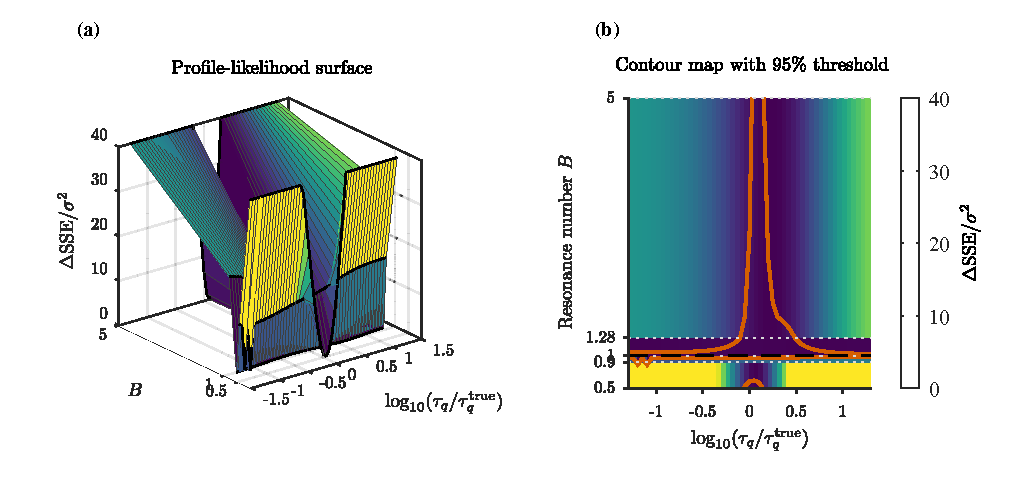
\includegraphics[width=\textwidth]{fig06_profile_surface_3d.pdf}
  \caption{Profile likelihood over the parameter plane $(\Bnum,\tq)$. (a) Three-dimensional profile-likelihood surface of $\Delta\mathrm{SSE}/\sigma^{2}$ over the $265$ computed points, five values of $\Bnum$ by $53$ values of $\tq$. The resonance number is drawn on its true numerical axis, the black curves mark the five computed rows, and no value is interpolated in $\Bnum$; the surface is clipped at $40$ for display only. (b) The same data as a contour map with the $95\%$ threshold $\chi^{2}_{1}=3.841$ marked. The admissible interval in $\tq$ widens without bound as $\Bnum\to1$: the width factor is $1.41$ at $\Bnum=0.5$, $3.55$ at $\Bnum=1.28$ and $1.26$ at $\Bnum=5$, while at $\Bnum=1$ the profile stays below the threshold across the whole grid. The row at $\Bnum=0.9$ is multimodal, because the re-optimisation at fixed $\tq$ reaches different local minima at adjacent nodes, and no interval is quoted from it.}
  \label{fig:profile}
\end{figure}


The row at $\Bnum = 0.90$ is reported separately because it is not a clean
profile. The re-optimisation over $(\alpha,\kk)$ at fixed $\tq$ converges to
different local minima at adjacent grid nodes, so the computed curve is not
unimodal and its lowest point falls at $0.08$ times the true relaxation time
rather than near it. A width factor read off such a curve would not be a
confidence interval, and none is quoted here. The failure is itself diagnostic:
at $\Bnum = 0.90$ the objective in the $(\tq,\kk)$ plane is already flat enough,
over more than an order of magnitude in $\tq$, that a two-start local optimiser
does not reliably locate the conditional optimum. The corresponding Fisher and
Monte Carlo standard errors at this condition, $98.8\%$ and $103.9\%$, are
obtained without re-optimisation and are unaffected. The profile rows at the
remaining four conditions are unimodal and are the ones used in the argument.

The factor of $3.55$ at $\Bnum = 1.28$ is the conditioning of a real
calibration, and it brackets the factor of $1.51$ to $3.50$ by which two
published evaluations of the same basalt specimens disagree, as discussed in
\cref{sec:cal-discrepancy}.




\subsection{Width of the ill-conditioned band}
\label{sec:prac-band}

Inverting the Fisher standard error as a function of $\Bnum$ gives the region
within which $\tq$ cannot be recovered to a stated precision:
%
\begin{align}
  \text{s.e.}(\tq) > 10\%  &: \quad \Bnum \in [0.441,\ 3.464] ,
  \label{eq:band10} \\
  \text{s.e.}(\tq) > 20\%  &: \quad \Bnum \in [0.628,\ 1.804] ,
  \label{eq:band20} \\
  \text{s.e.}(\tq) > 50\%  &: \quad \Bnum \in [0.817,\ 1.252] ,
  \label{eq:band50} \\
  \text{s.e.}(\tq) > 100\% &: \quad \Bnum \in [0.901,\ 1.116] .
  \label{eq:band100}
\end{align}
%
The exact degeneracy at a point therefore expands into a band of substantial
width. At the $20\%$ criterion the relaxation time is not usefully recoverable
anywhere in $\Bnum \in [0.628, 1.804]$, a range spanning nearly a factor of
three. These boundaries are properties of the configuration of
\cref{sec:prac-config}; the singularity at their centre is not.

\subsection{Well-determined parameter combinations}
\label{sec:prac-constructive}

The preceding results are negative statements about $\tq$ and $\kk$
individually. They are not statements about the informativeness of the data,
and it would be wrong to conclude that a measurement near resonance is
worthless. \Cref{tab:identifiability} also reports the standard errors of
$\alpha$ and of $\Bnum$ in the parameterisation \eqref{eq:reparam}. Across the
whole range, including exactly at $\Bnum = 1$, the diffusivity is determined to
about $1\%$ and the resonance number to between $4\%$ and $10\%$. The
information content of the record is essentially undiminished near resonance;
what fails is the resolution of a well determined combination into its two
components.

This is the constructive form of the result. Reporting $(\alpha, \Bnum)$, with
$\tq$ and $\kk$ quoted jointly rather than as independent point estimates, is
well posed everywhere. Reporting $\tq$ and $\kk$ as separate material constants
is not well posed for a material whose $\Bnum$ lies in the band
\eqref{eq:band20}. The recommendation of \cref{sec:design} follows directly.

\subsection{Optimiser dependence}
\label{sec:prac-optimiser}

Because the objective develops a long flat valley near resonance, the
estimate may depend on where the optimiser is started; this dependence is
real but, in the tests reported in \ref{app:optimiser}, smaller than the
effect of measurement noise itself, motivating multi-start or global search
strategies in poorly conditioned regimes.

%======================================================================
\section{Model Selection}
\label{sec:modelselection}

The identifiability result can be reached by a second, statistically
independent route. If at $\Bnum = 1$ the Guyer--Krumhansl response is
observationally a Fourier response, then a model selection criterion applied to
Guyer--Krumhansl data at resonance should prefer the Fourier model, because the
two extra parameters purchase no improvement in fit while incurring a
complexity penalty. That prediction is tested below.

\subsection{Candidate models and protocol}
\label{sec:ms-protocol}

The four candidates are exact special cases of the single transfer function
\eqref{eq:m2}, obtained by constraining parameters as derived in
\cref{sec:model-limits}: Fourier ($\tq=0$, $\kk=0$, $k=1$ parameter), the
Maxwell--Cattaneo--Vernotte model ($\kk = 0$, $k=2$), the Nyíri model
($\tq = 0$, $k=2$) and the full Guyer--Krumhansl model ($k=3$). Because all
four share one transfer function, they also share the solver, the estimation
procedure, the convergence criteria and the noise model; no model receives
individual tuning. This is what makes the comparison like for like.

The Maxwell--Cattaneo--Vernotte and Nyíri models are included because they
isolate the two mechanisms of the Guyer--Krumhansl equation separately, so the
comparison tests which mechanism the data require rather than merely whether
more parameters fit better. Models requiring a state variable absent from
\eqref{eq:m2}, such as those introducing a thermal displacement, are excluded:
they cannot be expressed as constraints on \eqref{eq:m2} and including them
would break the like for like protocol. This exclusion is stated rather than
passed over silently.

Selection uses the Bayesian information criterion of \cref{sec:methods-stats},
averaged over $15$ noise realisations at each condition, with data generated by
the full Guyer--Krumhansl model at $2\%$ noise. The Bayesian information
criterion is used in preference to the Akaike information criterion because
its stronger parsimony penalty gives the more conservative demonstration that
the rank deficiency of \cref{prop:main} is recoverable from a selection
statistic alone, without reference to any derivative or Fisher-matrix
information.

\subsection{Information-criterion scores}
\label{sec:ms-results}

The outcome is reported in \cref{tab:bic} and \cref{fig:bic}. Away from resonance the Guyer--Krumhansl
model is selected decisively, and increasingly so as $\Bnum$ moves away from
unity: at $\Bnum = 5.0$ the Fourier model is penalised by $267$ BIC units. At
$\Bnum = 1.00$ the ordering reverses and the Fourier model is selected, with
the Guyer--Krumhansl model penalised by $6.64$ units despite the data having
been generated by the Guyer--Krumhansl model itself.

The reversal is the expected behaviour of the criterion rather than a
limitation of it.
\begin{figure}[htbp]
  \centering
  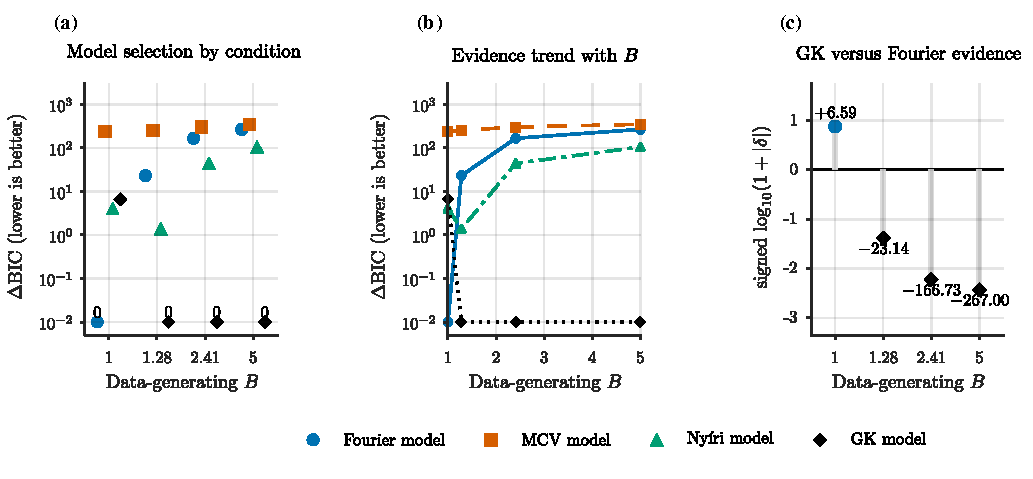
\includegraphics[width=\textwidth]{fig09_model_comparison.pdf}
  \caption{Like-for-like model comparison over the four nested candidates, each an exact special case of the single transfer function: the Fourier model ($k=1$ parameter), the Maxwell--Cattaneo--Vernotte model ($k=2$), the Ny\'iri model ($k=2$) and the Guyer--Krumhansl model ($k=3$). The criterion $\Delta\mathrm{BIC}$ is referenced to the best-scoring model at each condition, so lower values indicate stronger support and the selected model scores zero. (a) $\Delta\mathrm{BIC}$ by data-generating condition on a logarithmic ordinate; exact zeros are annotated explicitly because a logarithmic axis cannot represent zero. (b) Trend of the evidence with $\Bnum$. (c) Signed difference $\delta=\Delta\mathrm{BIC}_{\mathrm{GK}}-\Delta\mathrm{BIC}_{\mathrm{Fourier}}$, plotted as $\operatorname{sign}(\delta)\log_{10}(1+|\delta|)$ so that all four conditions remain visible across three orders of magnitude, with the exact values printed. A positive value indicates that the Fourier model is preferred even though the data were generated by the Guyer--Krumhansl model, which occurs at $\Bnum=1$. Synthetic data at $2\%$ noise, $15$ realisations per condition, identical estimation protocol for every candidate.}
  \label{fig:bic}
\end{figure}

\begin{table}[htbp]
  \centering
  \caption{Bayesian information criterion differences relative to the best
           model at each condition, averaged over 15 noise realisations. Data
           generated by the Guyer--Krumhansl model at 2\% noise; all four
           candidates are special cases of \eqref{eq:m2} fitted with an
           identical protocol. Lower is better; $0.00$ marks the selected
           model. The values are those of the frozen reference calculation.
           Four of the sixteen tabulated entries -- MCV and GK at
           $\Bnum=1.00$ ($236.58$ and $6.64$) and MCV at $\Bnum=1.28$ and
           $\Bnum=5.00$ ($253.21$ and $349.25$) -- are reproduced by
           independent re-evaluation with the production convolution solver
           during cross-platform validation as $240.31$ and $6.59$ at
           $\Bnum=1.00$ and as $253.63$ and $349.26$ at $\Bnum=1.28$ and
           $\Bnum=5.00$ respectively; the remaining twelve of sixteen entries
           agree to the digits shown. The differences arise in the two- and
           three-parameter fits at $\kk\to0$, where the two implementations of
           \eqref{eq:m2} differ by $O(10^{-12})$ and the
           Levenberg--Marquardt iteration amplifies that difference into the
           reported sum of squares. No model ranking, selection or conclusion
           is affected.}
  \label{tab:bic}
  \small
  \begin{tabular}{@{}rrrrrl@{}}
    \toprule
    \textbf{True} $\Bnum$ & \textbf{Fourier} & \textbf{MCV} &
    \textbf{Nyíri} & \textbf{GK} & \textbf{Selected} \\
    \midrule
    \textbf{1.00} & \textbf{0.00} & 236.58 & 4.03 & 6.64 & \textbf{Fourier} \\
    1.28 & 23.14  & 253.21 & 1.38   & \textbf{0.00} & GK \\
    2.41 & 166.73 & 302.12 & 44.21  & \textbf{0.00} & GK \\
    5.00 & 267.00 & 349.25 & 105.29 & \textbf{0.00} & GK \\
    \bottomrule
  \end{tabular}
\end{table}
 At resonance the two models make identical predictions, by
\cref{prop:cancel}, so the additional parameters reduce the residual only by
fitting noise and the parsimony penalty rejects them. The rank deficiency of
\cref{prop:main} is thereby recovered by a route that uses no derivative
information and no Fisher matrix.


The Maxwell--Cattaneo--Vernotte model is rejected everywhere by a wide margin,
$237$ to $349$ BIC units, consistent with the finding of Feh\'er and Kov\'acs
that this model cannot describe such experiments \cite{FeherKovacs2021}. The
Nyíri model, which retains the nonlocal term and discards relaxation, performs
far better than the Maxwell--Cattaneo--Vernotte model and is only marginally
worse than the full model near resonance. The ordering indicates that near
$\Bnum = 1$ the data do not require the relaxation mechanism.

\subsection{Statistical scope of the selection result}
\label{sec:ms-interp}

The Bayesian information criterion measures statistical parsimony under the
specified data generating process, noise model and observation design. It is
used here as an identifiability diagnostic and not as evidence about which
constitutive theory is physically correct. That the criterion prefers Fourier
at $\Bnum = 1$ is a statement about what the data can distinguish, not a
statement that the material obeys Fourier's law. This distinction matters when
interpreting model selection applied to real measurements: a Fourier
preference for a specimen near resonance is uninformative about the underlying
transport physics.


%======================================================================
\section{Implications for Published Calibrations}
\label{sec:calibration}

The preceding sections are statements about a model. The location of published
Guyer--Krumhansl calibrations relative to the identified ill-conditioned regime
is evaluated below, together with the consequences for the interpretation of the
reported values.

\subsection{Scope of the calibration audit}
\label{sec:cal-framing}

The interpretation of the aggregate calibration statistics requires
consideration of the admissible $\Bnum$-domain used in the source literature.
Feh\'er and Kov\'acs state that their
evaluation is restricted to the domain $1 \leq \Bnum < 3$, and identify its
lower limit with the Fourier case
\cite{FeherKovacs2021}. The accepted evaluation procedure therefore constrains
$\Bnum$ to an interval whose lower boundary is the exact degeneracy analysed in
\cref{sec:structural}. Values of $\Bnum$ close to unity in the literature are
in part a consequence of that admissible domain and of the physical
expectation, well supported by the measurements, that these materials behave
over diffusively. They reflect a structural property of the estimation
problem, not an incidental or coincidental property of the materials. The
restriction is well motivated: bounding a nonlinear search improves its
stability, and the domain reflects the observed regime.

\subsection{Audited calibrations}
\label{sec:cal-audit}

\Cref{tab:calibrations} lists all twelve Guyer--Krumhansl heat pulse
calibrations reported in \cite{Van2017,FeherKovacs2021} for which the
published parameters are sufficient to recompute $\Bnum$ from
\eqref{eq:Bdef}; no case meeting this criterion was excluded, and no
broader literature search beyond these two sources was undertaken. Every cell is flagged as reported by the original authors (R) or
calculated in the present study (C). Where the underlying parameters are
tabulated, $\Bnum$ was recomputed from \eqref{eq:Bdef}; the recomputed values
agree with the authors' own reported values to within $0.016$ in every case
where both exist, the largest deviation being for basalt at
\SI{3.84}{\milli\metre}. For the six basalt entries both the parameters and the
resulting $\Bnum$ were read directly from Tables~1 and~2 of
\cite{FeherKovacs2021}, which report the earlier and the refined evaluations
side by side.
\begin{table}[htbp]
  \centering
  \caption{Audited Guyer--Krumhansl calibrations. R denotes a value reported by
           the original authors; C denotes a value calculated in the present
           study from the reported parameters using \eqref{eq:Bdef}. The band
           is \eqref{eq:band20}, within which s.e.$(\tq)>20\%$ for the
           configuration of \cref{sec:prac-config}. Eleven of the twelve sources
           report no parameter uncertainty; case~12 is the exception.}
  \label{tab:calibrations}
  \scriptsize
  \resizebox{\textwidth}{!}{%
  \begin{tabular}{@{}rllrrrlc@{}}
    \toprule
    \# & \textbf{Source} & \textbf{Material} &
    $\alpha$ & $\tq$ & $\kk$ & $\Bnum$ & \textbf{In} \\
    & & & [\SI{e-6}{\metre\squared\per\second}] & [\si{\second}] &
    [\SI{e-6}{\metre\squared}] & & \textbf{band?} \\
    \midrule
    1  & V\'an et al.\ \cite{Van2017} & Capacitor \SI{3.9}{\milli\metre}
       & 2.13\,R & 0.954\,R & see note & 2.23\,R & no \\
    2  & V\'an et al.\ \cite{Van2017} & Limestone \SI{1.7}{\milli\metre}
       & 2.950\,R & 0.991\,R & see note & 2.17\,R & no \\
    3  & V\'an et al.\ \cite{Van2017} & Foam \SI{5.1}{\milli\metre}
       & 2.373\,R & 0.402\,R & see note & 3.04\,R & no \\
    4  & V\'an et al.\ \cite{Van2017} & Leucocratic \SI{1.75}{\milli\metre}
       & 4.77\,R & 1.32\,R & see note & 1.77\,R & \textbf{yes} \\
    \addlinespace
    5  & earlier eval. & Basalt \SI{1.86}{\milli\metre}
       & 0.55\,R & 0.738\,R & 0.509\,R & 1.243\,R / 1.254\,C & \textbf{yes} \\
    6  & earlier eval. & Basalt \SI{2.75}{\milli\metre}
       & 0.604\,R & 0.955\,R & 0.670\,R & 1.171\,R / 1.162\,C & \textbf{yes} \\
    7  & earlier eval. & Basalt \SI{3.84}{\milli\metre}
       & 0.68\,R & 0.664\,R & 0.480\,R & 1.060\,R / 1.063\,C & \textbf{yes} \\
    \addlinespace
    8  & Feh\'er \& Kov\'acs \cite{FeherKovacs2021} & Basalt \SI{1.86}{\milli\metre}
       & 0.61\,R & 0.211\,R & 0.168\,R & 1.295\,R / 1.305\,C & \textbf{yes} \\
    9  & Feh\'er \& Kov\'acs \cite{FeherKovacs2021} & Basalt \SI{2.75}{\milli\metre}
       & 0.61\,R & 0.344\,R & 0.268\,R & 1.272\,R / 1.277\,C & \textbf{yes} \\
    10 & Feh\'er \& Kov\'acs \cite{FeherKovacs2021} & Basalt \SI{3.84}{\milli\metre}
       & 0.68\,R & 1.000\,R & 0.650\,R & 0.940\,R / 0.956\,C & \textbf{yes} \\
    11 & Feh\'er \& Kov\'acs \cite{FeherKovacs2021} & Foam \SI{5.2}{\milli\metre}
       & 3.01\,R & 0.304\,R & 2.203\,R & 2.395\,R / 2.408\,C & no \\
    \addlinespace
    12 & Both et al.\ \cite{Both2016} & Capacitor \SI{3.9}{\milli\metre}
       & $1.958$\,R & $0.51$\,R & $1.53$\,R & 1.532\,C & \textbf{yes} \\
       & \multicolumn{7}{@{}l@{}}{\footnotesize\quad reported standard errors:
         $\pm0.004$, $\pm0.01$, $\pm0.03$ respectively; $R^{2}=0.9996$} \\
    \midrule
    \multicolumn{8}{@{}p{0.97\textwidth}@{}}{\footnotesize
      \textbf{Aggregate:} 8 of 12 inside the band \eqref{eq:band20} (all six
      basalt evaluations, the leucocratic rock at $\Bnum=1.77$ and the Both
      et al.\ capacitor at $\Bnum=1.53$); 4 of 12 outside.
      \textbf{Uncertainties:} eleven of the twelve report no parameter
      uncertainty. Case~12 \cite{Both2016} is the exception and reports
      standard errors from nonlinear regression
      ($\SI{0.2}{\percent}$ on $\alpha$, $\SI{2.0}{\percent}$ on $\tq$ and on
      $\kk$, $R^{2}=0.9996$); those errors are discussed in
      \cref{sec:cal-uncertainty}.
      \textbf{Note (cases 1--4):} the authors tabulate a length scale rather
      than $\kk$, and the reported dimensionless parameter could not be
      reproduced from it (limestone: 0.22\,C against 2.17\,R). The authors'
      reported values are used and the inconsistency is flagged, not
      reconciled. \textbf{Cases 5--7} were verified against Table~1 of
      \cite{FeherKovacs2021}, which tabulates the earlier values alongside the
      refined ones; the corresponding $\Bnum$ values are given in its
      Table~2.} \\
    \bottomrule
  \end{tabular}%
  }
\end{table}

\begin{figure}[htbp]
  \centering
  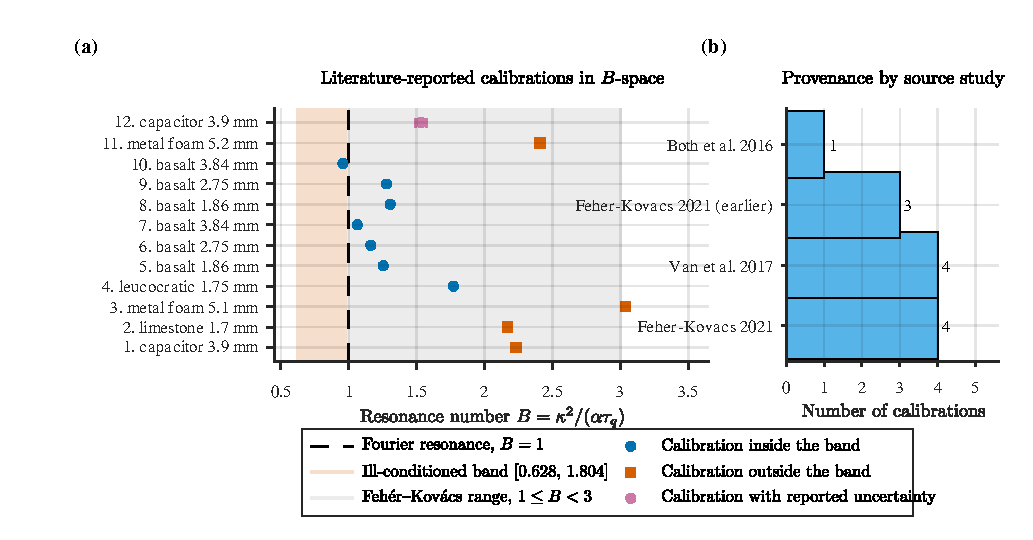
\includegraphics[width=\textwidth]{fig10_calibrations.pdf}
  \caption{Literature-reported Guyer--Krumhansl calibrations placed in $\Bnum$-space. (a) The twelve audited calibrations against the verified ill-conditioned band $\Bnum\in[0.628,1.804]$, within which $\mathrm{s.e.}(\tq)$ exceeds $20\%$, and against the range $1\leq\Bnum<3$ adopted by Feh\'er and Kov\'acs. Calibrations falling inside the band are drawn as blue circles and those outside as vermilion squares; eight of the twelve lie inside. Only one calibration reports parameter uncertainties and only that case carries an error bar. The remaining eleven source studies do not report uncertainties and none has been synthesised for them. (b) Provenance of the twelve calibrations across the four source studies.}
  \label{fig:calibrations}
\end{figure}


Eight of the twelve calibrations have $\Bnum$ inside the band
\eqref{eq:band20} within which the relaxation time carries a standard error
exceeding $20\%$ under the tested configuration, as shown in \cref{fig:calibrations}(a): all six basalt evaluations,
which cluster at $\Bnum = 0.94$ to $1.31$, the leucocratic rock at
$\Bnum = 1.77$, which falls just inside the upper edge, and the capacitor
evaluation of Both et al.\ at $\Bnum = 1.53$. The remaining four, comprising
the two metal foams, the limestone and the capacitor as evaluated by V\'an
et al., lie outside it at $\Bnum = 2.17$ to $3.04$. The ill-conditioned band is
therefore not a hypothetical construct: it contains a majority of the published
calibrations of this model, so the identifiability structure bears directly on
values already in circulation as material properties.


One feature of the audit requires explanation. V\'an et al.\ \cite{Van2017} use a different
nondimensionalisation from the one adopted here, scaling time by the pulse
length rather than by $L^{2}/\alpha$, and report a dimensionless group
$\hat{b} = \hat{\ell}^{2}/(\hat{\tau}\hat{\alpha})$ which is algebraically
identical to $\Bnum$. Combining their dimensionless table with their
dimensional table does not reproduce their $\hat{b}$: for limestone that route
gives $0.22$ against a reported $2.17$. Evaluated consistently within their
dimensionless table alone, however, $\hat{\ell}^{2}/(\hat{\tau}\hat{\alpha})$
returns $1.99$, $3.03$ and $1.78$ against reported values of $2.17$, $3.04$ and
$1.77$ for limestone, metal foam and leucocratic rock, agreeing to $0.01$ for
the latter two. The residual mismatch is traceable to the tabulated
$\hat{\alpha}$ for limestone and leucocratic rock, which differ from
$\alpha_{\mathrm{GK}} t_{p}/L^{2}$ computed from their own dimensional table by
factors of $9.1$ and $10.0$ respectively, while the capacitor and metal foam
entries agree to four significant figures. This is consistent with a units slip
confined to two rows of the published table. The authors' reported $\Bnum$
values are used here unchanged, and the two affected rows are flagged rather
than silently recomputed.

Eleven of the twelve calibrations report no parameter
uncertainty, correlation or confidence interval. The parameters are presented
as point estimates of material properties, and the present analysis indicates
that for eight of the twelve the relaxation time component of that estimate is
weakly constrained by the measurement used to obtain it, under the observation
design tested here. The single exception is treated separately in
\cref{sec:cal-uncertainty}.

\subsection{Calibration with reported uncertainties}
\label{sec:cal-uncertainty}

Both et al.\ \cite{Both2016} are the exception in the audited set. For the
layered capacitor they report standard errors from a nonlinear regression on
$2250$ data points: $\alpha = [1.958 \pm 0.004]\times10^{-6}\,
\si{\metre\squared\per\second}$, $\tq = [0.51 \pm 0.01]\,\si{\second}$ and
$\kk = [1.53 \pm 0.03]\times10^{-6}\,\si{\metre\squared}$, with
$R^{2} = 0.9996$. These correspond to relative standard errors of
$\SI{0.2}{\percent}$ on $\alpha$ and $\SI{2.0}{\percent}$ on both $\tq$ and
$\kk$, and place the specimen at $\Bnum = 1.53$, inside the band
\eqref{eq:band20}.

At first sight this contradicts the present analysis, which gives
$\SI{27}{\percent}$ on $\tq$ at $\Bnum = 1.53$. It does not, because the two
refer to different experiments. The band \eqref{eq:band20} is stated for the
configuration of \cref{sec:prac-config}, namely $80$ observations at
$\SI{2}{\percent}$ noise, whereas the cited regression uses $2250$ points at
substantially lower noise. Repeating the Fisher calculation at
$\Bnum = 1.532$ with $2250$ observations and $\SI{1}{\percent}$ noise returns a
standard error of $\SI{2.55}{\percent}$ on $\tq$, against the
$\SI{2.0}{\percent}$ reported. The agreement of these two independently
obtained figures is a check on the present framework against a real published
dataset, and it illustrates concretely why the band is described throughout as
configuration dependent rather than universal.

Two qualifications are needed. The reported standard errors are asymptotic
regression errors computed, as the authors state, assuming exact $L$ and
$t_{p}$; \cref{sec:practical} shows that such errors track Monte Carlo spread
well away from resonance but understate it close to it. And the specimen sits
at $\Bnum = 1.53$, near the upper edge of the band rather than at its centre;
the same measurement precision at $\Bnum \approx 1$ would not produce a
comparable result, since the degeneracy there is exact.

\subsection{Same-specimen discrepancy}
\label{sec:cal-discrepancy}

An independent consistency check is available, because three basalt specimens
were evaluated twice by different procedures. The two evaluations of the
identical specimens return relaxation times differing by a factor of up to
$3.50$ (Table~7). The refined evaluation reports
coefficients of determination above $0.99$ for all three specimens
\cite{FeherKovacs2021}; a directly comparable $R^{2}$ for the earlier
evaluation is not tabulated in the cited source and is not independently
verified here.
\begin{table}[htbp]
  \centering
  \caption{Two independent evaluations of the same three basalt specimens.
           The refined evaluation reports $R^{2}>0.99$ for the
           Guyer--Krumhansl fit for all three specimens; a comparable value is
           not tabulated for the earlier evaluation. All six lie at
           $\Bnum=0.94$ to $1.31$.}
  \label{tab:discrepancy}
  \small
  \begin{tabular}{@{}lrrrr@{}}
    \toprule
    \textbf{Specimen} & $\tq$ earlier [\si{\second}] &
    $\tq$ refined [\si{\second}] & \textbf{Ratio} &
    $R^{2}$ (refined) \\
    \midrule
    Basalt \SI{1.86}{\milli\metre} & 0.738 & 0.211 & $3.50\times$ & 0.9975 \\
    Basalt \SI{2.75}{\milli\metre} & 0.955 & 0.344 & $2.78\times$ & 0.9964 \\
    Basalt \SI{3.84}{\milli\metre} & 0.664 & 1.000 & $1.51\times$ & 0.9986 \\
    \bottomrule
  \end{tabular}
\end{table}


Two evaluations of the same data, each fitting well, returning relaxation times
that differ by up to a factor of three is precisely the signature of a flat
direction in the objective function. The magnitude is consistent with the
present analysis: all six evaluations sit at $\Bnum = 0.94$ to $1.31$, where
the Monte Carlo of \cref{sec:practical} gives central $90\%$ ranges for $\tq$
spanning factors of several to several tens, comfortably encompassing the
observed spread.

The causal claim must nonetheless be limited. The observed parameter spread is
consistent with and quantitatively accounted for by the identifiability
structure near $\Bnum \approx 1$, while differences in pulse modelling,
smoothing, and fitting procedures may also contribute. The two evaluations
differ in more than one respect, and the present data do not permit the
contributions to be separated. It is not claimed that the degeneracy caused the
discrepancy.



%======================================================================
\section{Implications for Measurement Design}
\label{sec:design}

The analysis converts into a design criterion. Inverting the Fisher standard
error of \cref{sec:practical} gives, for each target precision on $\tq$, the
region of $\Bnum$ in which that target is attainable:
%
\begin{align}
  \text{s.e.}(\tq) \leq 10\% &:\quad
    \Bnum \leq 0.441 \ \text{ or }\ \Bnum \geq 3.464 ,
  \label{eq:design10} \\
  \text{s.e.}(\tq) \leq 20\% &:\quad
    \Bnum \leq 0.628 \ \text{ or }\ \Bnum \geq 1.804 ,
  \label{eq:design20} \\
  \text{s.e.}(\tq) \leq 30\% &:\quad
    \Bnum \leq 0.723 \ \text{ or }\ \Bnum \geq 1.468 ,
  \label{eq:design30} \\
  \text{s.e.}(\tq) \leq 50\% &:\quad
    \Bnum \leq 0.817 \ \text{ or }\ \Bnum \geq 1.252 .
  \label{eq:design50}
\end{align}
%
These boundaries hold for the configuration of \cref{sec:prac-config} and are
not universal constants. They should be recomputed for any materially different
observation design. The qualitative structure, an excluded interval centred on
$\Bnum = 1$ whose width grows as the precision target tightens, is universal,
because it follows from the structural result of \cref{sec:structural}.

\subsection{Adjustable and fixed design variables}
\label{sec:design-levers}

$\Bnum$ is composed of material properties and is not a free instrument
setting. The available levers are correspondingly limited, and one commonly
assumed lever does not exist.

\paragraph{Material selection.}
The most effective lever is the choice of specimen. The audited calibrations of
\cref{sec:calibration} indicate that metal foams, at $\Bnum \approx 2.4$ to
$3.0$, and the limestone and capacitor samples at $\Bnum \approx 2.2$, are far
better conditioned for relaxation time estimation than basalt at
$\Bnum \approx 0.94$ to $1.31$ or the leucocratic rock at $\Bnum = 1.77$. A preliminary estimate of $\Bnum$ should
therefore precede any campaign whose objective is to report $\tq$.

\paragraph{Operating temperature.}
The three coefficients $\alpha$, $\tq$ and $\kk$ are all temperature dependent,
so $\Bnum$ shifts with operating temperature. This provides a genuine, if
material specific, means of moving a specimen away from resonance.

\paragraph{Specimen thickness does not move $\Bnum$.}
This point is emphasised because the opposite is easy to assume. By
\eqref{eq:B-invariance}, $\Bnum$ is invariant under the scaling
\eqref{eq:param-scaling}: the thickness cancels identically, and within the
present one dimensional model all thicknesses of a given material share one
value of $\Bnum$. This is confirmed by the audited data, where three basalt
specimens of \SI{1.86}{}, \SI{2.75}{} and \SI{3.84}{\milli\metre} yield the
same $\Bnum$ to three significant figures from a single parameter set. Varying
the thickness therefore cannot be used to escape the ill-conditioned band.

\paragraph{Multiple thicknesses as independent records.}
What multiple thicknesses do provide is additional independent observations of
the same material, which reduces the variance of a joint inversion in the
ordinary way. This is a replication benefit, not a change in $\Bnum$, and it
does not remove the structural degeneracy: at exactly $\Bnum = 1$ every record,
at every thickness, is a Fourier record, so no number of them separates $\tq$
from $\kk$.

\paragraph{Sampling and noise.}
Denser sampling during the rise, where the sensitivity to $\tq$ is
concentrated, and lower noise both reduce the standard error roughly in
proportion to the usual factors, and so shift the band boundaries modestly
inward. Neither removes the singularity, which is independent of noise level
and sampling density by \cref{def:struct}.

\subsection{Recommended reporting practice}
\label{sec:design-recommendation}

The single most useful change to reporting practice is inexpensive: report
$\Bnum$ alongside every fitted $(\tq, \kk)$ pair. It is computed directly from
the fitted parameters by \eqref{eq:Bdef}, requires no additional measurement,
and tells a reader immediately whether the reported relaxation time is
supported by the data or is a point on a flat valley. Where $\Bnum$ falls
inside the band, the parameters should be reported in the $(\alpha, \Bnum)$
form of \eqref{eq:reparam}, with an interval rather than a point estimate for
$\tq$. \Cref{tab:design} summarises the admissible $\Bnum$ for each target
precision together with the material classes of the audited set that satisfy
it.
\begin{table}[htbp]
  \centering
  \caption{Measurement design criterion. Admissible $\Bnum$ for a target
           standard error on $\tq$, for the configuration of
           \cref{sec:prac-config}. These are not universal constants and
           should be recomputed for a different design. Thickness is not a
           lever: $\Bnum$ is invariant under \eqref{eq:B-invariance}.}
  \label{tab:design}
  \small
  \resizebox{\textwidth}{!}{%
  \begin{tabular}{@{}lll@{}}
    \toprule
    \textbf{Target s.e.}$(\tq)$ & \textbf{Admissible} $\Bnum$ &
    \textbf{Example material class} \\
    \midrule
    $\leq 10\%$ & $\Bnum \leq 0.441$ or $\Bnum \geq 3.464$ &
      none of the audited set \\
    $\leq 20\%$ & $\Bnum \leq 0.628$ or $\Bnum \geq 1.804$ &
      metal foams, capacitor, limestone \\
    $\leq 30\%$ & $\Bnum \leq 0.723$ or $\Bnum \geq 1.468$ &
      the above, plus leucocratic rock \\
    $\leq 50\%$ & $\Bnum \leq 0.817$ or $\Bnum \geq 1.252$ &
      the above, plus basalt at \SI{1.86}{} and \SI{2.75}{\milli\metre} \\
    \bottomrule
  \end{tabular}%
  }
\end{table}



%======================================================================
\section{Discussion}
\label{sec:discussion}

The principal finding is that a coincidence between two constitutive models,
already known at the level of their solutions, has a consequence at the level
of the inverse problem that does not follow from it automatically and that
changes how published Guyer--Krumhansl coefficients should be read. The
following subsections separate what was already established from what the
present analysis adds, relate the structural and practical statements, and set
out the consequences for calibration practice.

\subsection{Established cancellation and its inverse-problem consequence}
\label{sec:disc-known}

The Fourier resonance itself is established
\cite{Kovacs2018,FulopKovacsVan2015,Fulop2018entropy,FeherKovacs2021}; no
priority is claimed for it here. What this paper adds is the inverse-problem
consequence: that two models coincide on a surface in parameter space is a
statement about solutions, whereas the coincidence rendering a parameter pair
unrecoverable from any temperature observation is a statement about the
parameter-to-observable map, and the second does not follow from the first
without the sensitivity analysis of \cref{sec:structural}. The specific
additions are the exact anti-parallel sensitivity relation
\eqref{eq:antiparallel} with its null direction $(1,\alpha)$, the consequent
rank deficiency and Fisher singularity, the quantified width of the
surrounding ill-conditioned region, the identification of $(\alpha,\Bnum)$ as
the combination the data determine, and the resulting implications for
calibration practice, model selection and measurement design.

\subsection{Structural and practical identifiability}
\label{sec:disc-struct-prac}

The two notions behave differently and the distinction carries the argument.
The structural result is exact, holds at a single point, and is independent
of noise, sampling and estimator; the practical result is approximate, holds
over a finite region, and depends on all three. Neither alone would be
sufficient: a point singularity in a three-parameter space would be a measure
zero curiosity, while large standard errors without the exact result could
always be attributed to an inadequate optimiser. It is the combination -- an
exact degeneracy at $\Bnum=1$ broadening continuously into the band
\eqref{eq:band20} -- that makes the finding relevant to real calibrations,
eight of the twelve audited here lying inside that band.

\subsection{Reparameterisation rather than abandonment}
\label{sec:disc-reparam}

The results are not an argument against the Guyer--Krumhansl model: it
reproduces the measurements well, and the diffusivity and resonance number
are recovered to about $1\%$ and $10\%$ even at the singularity itself. What
fails is a specific act of interpretation -- quoting $\tq$ and $\kk$ as
independent material constants when the observation constrains only a
combination of them. The remedy is to report the combination the data
determine, which is why \cref{sec:model-param} introduces \eqref{eq:reparam}
as a device of the analysis rather than as a discovery.

\subsection{Model-selection evidence}
\label{sec:disc-bic}

The Bayesian information criterion reaches the same conclusion by a route
using neither derivatives nor a Fisher matrix: selecting the Fourier model at
$\Bnum=1$ from Guyer--Krumhansl-generated data is the rank deficiency
expressed statistically, since the criterion cannot distinguish the
additional parameters from the Fourier limit under the resonance condition.
For experimentalists this is a caution rather than a diagnostic: a model
comparison performed near resonance favours the simpler model regardless of
the underlying physics, so a Fourier preference in that regime is evidence
about the design, not the material.

\subsection{Implications for published calibrations}
\label{sec:disc-calibration}

The appropriate inference from the audited calibrations is about precision
rather than correctness. The reported basalt relaxation times are not shown
to be wrong; they are shown to be weakly constrained by the measurements from
which they were obtained, whereas the reported diffusivities are well
constrained throughout. This is consistent with, though not established as
caused solely by, the identified degeneracy, since the two basalt evaluations
also differ in pulse model, smoothing and fitting procedure.

The single calibration reporting uncertainties provides a check in the
opposite direction: Both et al.\ \cite{Both2016} quote $\SI{2.0}{\percent}$
on $\tq$ at $\Bnum=1.53$, and the present framework, evaluated at their
sampling density and noise level, returns $\SI{2.55}{\percent}$. Two
independently obtained estimates agreeing at this level support the Fisher
construction used throughout and show that a specimen inside the band can
still yield a precise relaxation time given a sufficiently informative
measurement -- the band identifies where precision is expensive, not where it
is unattainable.

\subsection{Conditions under which the pair is separable}
\label{sec:disc-separable}

Separation requires the material to sit away from resonance, by a distance
set by the target precision: for the design of \cref{sec:prac-config}, a
$20\%$ standard error on $\tq$ requires $\Bnum\leq0.628$ or
$\Bnum\geq1.804$, and a $10\%$ error requires $\Bnum\leq0.441$ or
$\Bnum\geq3.464$ -- satisfied by no specimen in the audited set. Two levers
act on this condition: specimen selection, since $\Bnum$ is a material
property (the metal foams of the audited set, at $\Bnum\approx2.4$--$3.0$,
are the best-conditioned available), and measurement quality, which shifts
the band boundaries without moving $\Bnum$ (the capacitor calibration of
Both et al.\ \cite{Both2016} attains $2.0\%$ at $\Bnum=1.53$, inside the
reference $20\%$ band, using $2250$ low-noise observations). Specimen
thickness is not a lever, since $\Bnum$ is invariant under
\eqref{eq:B-invariance}. The practical criterion is therefore to estimate
$\Bnum$ from a preliminary fit before committing to a relaxation-time
measurement.

\subsection{Regime of validity}
\label{sec:disc-regime}

The analysis concerns the Guyer--Krumhansl equation as an effective continuum
description of heterogeneous media at room temperature, with coefficients
constrained by the second law rather than derived from a carrier model
\cite{Van2001,Van2017} -- the regime of the audited calibrations.
Conclusions are not extended to the phonon-hydrodynamic regime in dielectric
crystals at low temperature, where the coefficients have a kinetic
interpretation obtainable independently of a flash-experiment fit and the
inverse problem examined here does not arise in the same form.

%======================================================================
\section{Scope and Limitations}
\label{sec:limitations}

\paragraph{One-dimensional formulation.}
The analysis is carried out for the one dimensional slab of \cref{sec:model}.
The cancellation of \cref{prop:cancel} is a property of the propagation factor
$m^{2}(s)$, which arises in the same form in geometries that separate, so the
structural result is expected to persist there; a treatment of genuinely
multi dimensional geometries, including lateral losses and finite beam
profiles, has not been carried out and is not claimed.

\paragraph{Inverse experiments are synthetic.}
The identifiability results are established on synthetic data. This is
necessary rather than incidental: demonstrating that two parameter sets are
indistinguishable requires knowing the parameter values that generated the
data, which no experiment provides. The synthetic study is anchored to reality
by using physical basalt parameters, by auditing published calibrations in
\cref{sec:calibration}, and by the same specimen discrepancy of
\cref{tab:discrepancy}, which is real data behaving as the analysis predicts.
It remains a limitation that the inverse conclusions have not been tested
against a controlled experiment with independently known parameters.

\paragraph{The band is configuration dependent.}
The numerical boundaries \eqref{eq:band10}--\eqref{eq:band100} and the design
criterion \eqref{eq:design10}--\eqref{eq:design50} hold for the configuration
of \cref{sec:prac-config}. They are not physical constants and would move under
a different sampling scheme, noise level, or pulse length. Only the singularity
at $\Bnum = 1$ is universal.

\paragraph{Forward validation is not inverse validation.}
\cref{sec:validation} validates the forward operator against published figures.
It does not validate the inverse problem, and is not offered as doing so. The
inverse results rest on the analytical proof of \cref{sec:structural} together
with the numerical certification of \cref{sec:certification} and the
independent statistical route of \cref{sec:modelselection}.

\paragraph{Dependence on the pulse and boundary model.}
The structural result is independent of the excitation, since $\hat{Q}_{0}(s)$
cancels from the sensitivity ratio \eqref{eq:ratio-chain}. The width of the
practically ill-conditioned band is not: it depends on the pulse shape and
duration through the information content of the record. Boundary cooling,
neglected here as in the anchor, would modify the observable and hence the band
boundaries, though not the degeneracy.

\paragraph{Unverified bibliographic and calibration items.}
For the four samples of V\'an et al.\ the reported dimensionless parameter
could not be reproduced from the tabulated length scale, as recorded in
\cref{sec:cal-audit}; the discrepancy is flagged and not reconciled. The three
earlier basalt evaluations were verified against Table~1 of
\cite{FeherKovacs2021}, which reproduces them; they were not traced further
back to the measurement report in which they originally appeared.
Sections~4 and~5 of the version of record of the anchor are behind a paywall,
and the equations used here were transcribed from the open preprint; the
version of record is Volume~127, Part~A, and its equation numbering differs
from the preprint, which is why no equation numbers of the anchor are cited in
\cref{sec:model-anchor}.

\paragraph{Raw experimental data unavailable.}
The published heat pulse time series underlying the audited calibrations are
not available, so the re-analysis of \cref{sec:calibration} necessarily works
from tabulated fitted values rather than from the measurements themselves. A
direct re-inversion of the original records, with uncertainty quantification,
would be a stronger test and is not possible with the published material.

\paragraph{Literature screening was not performed on an authenticated citation index.}
Access to Scopus and Web of Science was not available. The screening reported
in \cref{sec:introduction} used open bibliographic sources with validated positive
controls, covered title and abstract records rather than full text, and
achieved abstract coverage of about $60\%$ of the retrieved corpus. Statements
about the absence of prior work are therefore statements about the screened
corpus and not absolute priority claims. An authenticated index search remains
outstanding.

\paragraph{Local optima in the profile computation.}
The profile likelihood is computed by re-optimising the remaining parameters at
each node of a fixed $\tq$ grid with a two-start local method. At
$\Bnum = 0.90$ this procedure does not return a unimodal profile, as recorded in
\cref{sec:prac-profile}, so no confidence interval is quoted at that condition.
A global search at each node would resolve it. The conclusions rest on the four
conditions at which the profile is unimodal, on the Fisher analysis and on the
Monte Carlo study, none of which requires re-optimisation at fixed $\tq$.

\paragraph{A superseded numerical result.}
As detailed in \ref{app:optimiser}, an earlier implementation produced a
larger optimiser-initialisation effect than the certified solver reproduces;
that earlier result is not used. Similarly, an earlier reported discrepancy
between Fisher and Monte Carlo uncertainties was traced to finite-difference
Jacobians and withdrawn; \cref{sec:practical} reports agreement between the two
where the asymptotic approximation is valid.

%======================================================================
\section{Conclusions}
\label{sec:conclusions}

The parameter-to-observable map of the one-dimensional Guyer--Krumhansl heat
pulse problem has been analysed as an inverse problem, using a Laplace-domain
convolution solver with analytic sensitivities, cross-checked against an
independent finite-difference scheme and an arbitrary-precision reference, and
externally validated against three published figures of an independently
authored analytical solution at normalised errors of $0.384\%$, $0.382\%$ and
$0.483\%$ with no parameter fitting.

Three findings follow. First, at the Fourier resonance
$\Bnum = \kk/(\alpha\tq) = 1$, a condition established in the existing
literature and not claimed here, the response is independent of the relaxation
time at every position and time and for any excitation; the sensitivities
satisfy $\partial T/\partial \tq = -\alpha\,\partial T/\partial \kk$ exactly, so
the sensitivity matrix has rank one with null direction $(1,\alpha)$, the Fisher
matrix is singular, and $\tq$ and $\kk$ are structurally non-identifiable from
any temperature record at any noise level or sampling density. Second, the
degeneracy is not confined to that point: for the tested configuration the
relaxation time carries a standard error above $20\%$ throughout
$\Bnum \in [0.628, 1.804]$ and above $50\%$ throughout
$\Bnum \in [0.817, 1.252]$; at $\Bnum=1$ specifically, within this
ill-conditioned region, the Bayesian information
criterion selects the Fourier model over the Guyer--Krumhansl model even for
Guyer--Krumhansl data, while away from resonance the Guyer--Krumhansl model is
selected decisively at every tested condition, including $\Bnum=1.28$ inside
the $20\%$ band. Third, the record nevertheless remains informative: the
diffusivity is recovered to about $1\%$ and the resonance number to between
$4\%$ and $10\%$ across the whole range including exactly at resonance, so what
fails is the resolution of a determined combination into two coefficients rather
than the determination of the transport behaviour.

The contribution is therefore a statement about estimation rather than
constitutive modelling: a coincidence already known at the level of
solutions is shown to impose an exact rank deficiency on the inverse
problem, with the neighbourhood in which that deficiency dominates
finite-noise estimation quantified. The practical consequence is concrete:
of twelve audited published calibrations, eight lie inside the band and
eleven report no parameter uncertainty, and two independent evaluations of
the same three basalt specimens return relaxation times differing by
factors of $1.51$ to $3.50$ at $R^{2}>0.99$, consistent with, though not
attributable solely to, the identified structure. Guyer--Krumhansl
coefficients are best reported in the $(\alpha,\Bnum)$ parameterisation, and
campaigns targeting the relaxation time should select specimens away from
resonance, since specimen thickness leaves $\Bnum$ invariant.

The analysis is confined to the one-dimensional slab and to synthetic inverse
experiments; the band boundaries are properties of the stated observation design
and only the singularity at their centre is universal. No experimental
validation of the inverse conclusions is claimed. The most useful extension is a
controlled heat pulse experiment on a specimen of independently determined
$\Bnum$, which would test the predicted precision directly and, for a specimen
placed away from resonance, establish whether the relaxation and nonlocal
coefficients can be separated in practice at the precision the present analysis
predicts.

%======================================================================
\section*{CRediT authorship contribution statement}

\textbf{V. Gupta:} Conceptualization, Methodology, Software, Formal
analysis, Validation, Writing -- original draft, Writing -- review \&
editing.

%======================================================================
\section*{Declaration of competing interest}

The author declares that he has no known competing financial interests or
personal relationships that could have appeared to influence the work
reported in this paper.

%======================================================================
\section*{Data availability}

The numerical implementation, the MATLAB/Octave figure-generation scripts, and
the verified numerical results underlying every figure and table in this
paper are available from the corresponding author upon reasonable request.
[REPOSITORY DOI OR URL -- TO BE SUPPLIED BY AUTHOR upon deposit, e.g. Zenodo
or an institutional repository, prior to submission.]

\appendix

\section{Numerical Algorithm}
\label{app:algorithm}

Algorithm~\ref{alg:main} gives the complete procedure summarised in
\cref{sec:methods-algorithm}.

\begin{algorithm}[htbp]
\caption{Forward evaluation, sensitivity assembly and identifiability
         diagnostics for the Guyer--Krumhansl rear-face problem.}
\label{alg:main}
\begin{algorithmic}[1]
\Require diffusivity $\alpha$, relaxation time $\tq$, nonlocal coefficient
         $\kk$, slab thickness $L$, pulse length $t_p$, sample times
         $\{t_i\}_{i=1}^{n}$, noise level $\eta$
\Ensure  rear-face history $\hat{T}(1,t_i)$, Fisher matrix $F$, standard errors,
         profile likelihood, model-selection scores

\Statex \textbf{Stage 1: dimensionless reduction}
\State $B \gets \kk/(\alpha\tq)$, \;
       $\tau_{\Delta} \gets L^{2}/\alpha$, \;
       $\hat{t}_i \gets t_i/\tau_{\Delta}$
       \Comment{\cref{sec:model-nondim}}

\Statex \textbf{Stage 2: forward solution (Solver A)}
\State Form the propagation function
       $m^{2}(s) = s\,(1+\tq s)/(\alpha + \kk s)$
       \Comment{\cref{eq:m2}}
\State Factorise $\hat{T}(1,s) = \hat{K}(s)\,\hat{Q}_0(s)$ and retain
       \emph{only} $\hat{K}$ for numerical inversion
       \Comment{$\hat{Q}_0$ carries removable poles}
\State Invert $\hat{K}$ on a fixed Talbot contour with $M=41$ nodes
       \Comment{$M$ odd; see \cref{sec:cert-talbot}}
\State Convolve the inverted kernel with the analytic pulse $q_0$ by
       Gauss--Legendre quadrature, $n_q = 32$
\State \Return $\hat{T}(1,\hat{t}_i)$

\Statex \textbf{Stage 3: independent cross-checks}
\State Solve the same problem with Solver B, a staggered-grid finite-difference
       scheme at $N_x = 400$, and with Solver C at $50$-digit precision
\State \textbf{assert} pairwise agreement within the criteria of
       \cref{tab:certification}
       \Comment{numerical cross-checking, not external validation}

\Statex \textbf{Stage 4: analytic sensitivities}
\For{$\theta \in \{\alpha,\ \tq,\ \kk\}$}
  \State Differentiate $m^{2}(s)$ in closed form and invert
         $\partial\hat{K}/\partial\theta$ on the same contour
         \Comment{no finite differencing}
\EndFor
\State Assemble the Jacobian $J_{i\theta} = \partial \hat{T}(1,\hat{t}_i)/
       \partial\theta$

\Statex \textbf{Stage 5: identifiability diagnostics}
\State $F \gets \sigma^{-2} J^{\top} J$; evaluate
       $\operatorname{cond}(\tilde F)$, $\rho_{\tq\kk}$ and
       $\operatorname{s.e.}(\theta) = \sqrt{[F^{-1}]_{\theta\theta}}$
\If{$\operatorname{cond}(\tilde F) > 10^{12}$}
  \State report the pair as numerically non-identifiable at this $\Bnum$
\EndIf
\State Profile the likelihood in $\tq$ on a fixed grid, re-optimising the
       remaining parameters at each node, and intersect with the
       $\chi^{2}_{1}$ threshold $3.841$
\State Repeat the estimation over $200$ Monte Carlo noise realisations and
       compare the sampling spread with the Fisher prediction

\Statex \textbf{Stage 6: model comparison}
\For{each candidate $\mathcal{M}\in\{$Fourier, MCV, Nyíri, GK$\}$}
  \State Fit $\mathcal{M}$ to the same synthetic record by
         Levenberg--Marquardt with three restarts
  \State $\mathrm{BIC}_{\mathcal{M}} \gets n\ln(\mathrm{SSE}/n) + k\ln n$
         \Comment{$k$ = number of free parameters}
\EndFor
\State $\Delta\mathrm{BIC} \gets \mathrm{BIC} - \min_{\mathcal{M}}\mathrm{BIC}$
       and select $\arg\min$
\end{algorithmic}
\end{algorithm}


\clearpage
\section{Notation Correspondence with the Validation Anchor}
\setcounter{table}{0}
\label{app:notation}

\Cref{tab:notation} lists the correspondence between the notation used
here and that of the validation anchor \cite{Kovacs2018}, referenced from
\cref{sec:model-anchor,sec:validation}.


\begin{table}[htbp]
  \centering
  \caption{Correspondence between the present notation and that of the
           validation anchor \cite{Kovacs2018}. Symbols are matched by the
           quantity they denote, not by appearance.}
  \label{tab:notation}
  \small
  \begin{tabularx}{\textwidth}{@{}llXl@{}}
    \toprule
    \textbf{Present} & \textbf{Anchor} & \textbf{Quantity} &
    \textbf{Conversion} \\
    \midrule
    $\alpha$              & $\alpha$            &
      thermal diffusivity $\lambda/(\rho c)$ & identical \\
    $\tq$                 & $\tau_{q}$          &
      relaxation time of the heat flux & identical \\
    $\kk$                 & $\kappa^{2}$        &
      coefficient of $\partial_{t}\partial_{xx}T$, dimension
      \si{\metre\squared} & identical \\
    $\tau_{\Delta}$       & $\hat{\tau}_{\Delta}$ &
      dimensionless pulse length & $\alpha t_{p}/L^{2}$ \\
    $\hat{\tau}_{q}$      & $\hat{\tau}_{q}$    &
      scaled relaxation time & $\alpha \tq/L^{2}$ \\
    $\hat{\kappa}^{2}$    & $\hat{\kappa}^{2}$  &
      scaled nonlocal coefficient & $\kk/L^{2}$; the anchor also
      writes $\hat{\kappa}=\kappa/L$ \\
    $\Bnum$               & $\kappa^{2}/(\alpha\tau_{q})$ &
      Fourier-resonance number; the anchor states the resonance as
      $\kappa^{2}/\tau_{q}=\alpha$ & $\Bnum = \kk/(\alpha\tq)$ \\
    $m(s)$                & not used            &
      Laplace propagation factor; the anchor uses an eigenfunction
      expansion & introduced here \\
    \bottomrule
  \end{tabularx}
\end{table}


\clearpage
\section{Supplementary Numerical Certification}
\setcounter{table}{0}
\label{app:certification}

\Cref{tab:certification} itemises the complete numerical error budget
underlying the certification summarised in \cref{sec:certification} and
illustrated in \cref{fig:talbot,fig:convergence}.


\begin{table}[htbp]
  \centering
  \caption{Numerical certification and error budget. Each entry states the
           scope over which it was established. Agreement between the present
           solvers is numerical cross-checking, not external validation.}
  \label{tab:certification}
  \small
  \begin{tabularx}{\textwidth}{@{}p{4.3cm}p{3.5cm}X@{}}
    \toprule
    \textbf{Item} & \textbf{Result} & \textbf{Scope} \\
    \midrule
    Talbot node parity
      & failure at $t^{\ast}=M\tau_{\Delta}/10$ for even $M$
      & split formulation; error $10^{9}$--$10^{11}$ at $t^{\ast}$,
        $10^{-4}$ adjacent; absent for odd $M$ \\
    \addlinespace
    Convolution formulation
      & no pole encountered
      & kernel $\hat{K}$ is pole free; adopted throughout \\
    \addlinespace
    Talbot node count
      & plateau $M\in[25,81]$; $M=41$ used
      & degrades beyond $M\approx 91$ by round off \\
    \addlinespace
    Convolution quadrature
      & $\leq 10^{-13}$
      & 32 versus 64 Gauss--Legendre nodes \\
    \addlinespace
    Solver A versus Solver C
      & $10^{-11}$ to $10^{-13}$
      & probe times away from the steep rise \\
    \addlinespace
    Solver A versus Solver B
      & $\approx 10^{-7}$
      & full record; limited by finite differences \\
    \addlinespace
    Finite difference, space
      & observed order $p=2.00$; $2.6\times10^{-6}$
      & $N_{x}=400$ against Richardson reference \\
    \addlinespace
    Finite difference, time
      & $\approx 10^{-9}$
      & relative tolerance $10^{-10}$ \\
    \addlinespace
    Arithmetic precision
      & $\leq 8.9\times10^{-16}$
      & 15, 30 and 50 digits compared \\
    \addlinespace
    Fourier-resonance limit
      & $2.6\times10^{-6}$
      & $\kk=\alpha\tq$ against analytical Fourier solution \\
    \addlinespace
    Non-negativity, steady state
      & $T \geq 0$; $T(\infty)=1.00000000$
      & all cases tested \\
    \addlinespace
    \textbf{Total numerical error}
      & $\approx 10^{-6}$
      & versus digitisation floor $6\times10^{-3}$ \\
    \bottomrule
  \end{tabularx}
\end{table}


\clearpage
\section{Optimiser-Initialisation Sensitivity}
\label{app:optimiser}

This appendix gives the complete optimiser-initialisation sensitivity study
summarised in \cref{sec:prac-optimiser}. Starting points were drawn from
log-normal perturbations of the true parameters at $\Bnum=1.277$, and the
spread of the recovered values was recorded separately from the spread
induced by measurement noise.

\begin{table}[htbp]
  \centering
  \caption{Optimiser-initialisation sensitivity at $\Bnum=1.277$. The central
           $90\%$ range of recovered $\tq$ and $\Bnum$ is reported as a
           multiple of the true value, for increasing perturbation of the
           optimiser starting point.}
  \label{tab:optimiser}
  \begin{tabular}{@{}lll@{}}
    \toprule
    \textbf{Perturbation} & \textbf{$\tq$ range (central 90\%)} & \textbf{$\Bnum$ range} \\
    \midrule
    $0.5$ log units & essentially unchanged & $0.91$ to $1.28$ \\
    $1.0$ log units & factor $4.7 \to 9.3$ & $0.91$ to $1.28$ \\
    \bottomrule
  \end{tabular}
\end{table}

With the certified solver the effect is modest and, in these tests, smaller
than the effect of measurement noise itself; a small number of realisations
converge to a distant local minimum rather than following the trend in the
table. Parameter estimates can nonetheless exhibit substantial dependence on
optimiser initialisation in poorly conditioned regimes, motivating multi-start
or global search strategies. An implementation of the Laplace inversion based
on the split pulse formulation, whose failure at $t^{\ast}=M\tau_{\Delta}/10$
is characterised in \cref{sec:cert-talbot}, exhibits a substantially larger
effect, a spread of roughly a factor of twenty-three in recovered $\tq$,
because for the settings then in use the failure time fell inside the
observation window; the result in the table, obtained with the certified
convolution solver, supersedes this and is the value used throughout the
paper.


\bibliographystyle{elsarticle-num}
\bibliography{references}

\end{document}
